%!TEX TS-program = xelatex
%!TEX encoding = UTF-8 Unicode

% Modify the following line to match your school
% Available options include `Harvard`, `Princeton`, and `NYU`.
\documentclass[School=UAB]{Dissertate}

\begin{document}

% frontpage and signatures

% Some details about the dissertation.
\title{GAUDI\textsubscript{ASM}\\\vspace{15pt}A novel tool for computationally aided molecular design}
\author{Jaime Rodríguez-Guerra Pedregal}
\advisor{Jean-Didier Maréchal}

% ... about the degree.
\degree{Bioinformatics}
\field{Structure and Function of \\Proteins and Drug Design}
\degreeyear{2014}
\degreemonth{September 1st,}
\department{Molecular Modeling of \\Transition Metal Systems}
\faculty{Chemistry}

% ... about the candidate's previous degrees.
\pdOneName{Degree in Biotechnology}
\pdOneSchool{University of Salamanca}
\pdOneYear{2013}

% \pdTwoName{M.A.}
% \pdTwoSchool{Monster's Univeristy}
% \pdTwoYear{2021}
\maketitle
\cleardoublepage
\abstractpage
\clearpage

%frontmatter
\pagenumbering{roman}
\setcounter{page}{2}
\tableofcontents
\clearpage
% \acknowledgments
% \cleardoublepage

% actual contents
\pagestyle{fancy}
\fancyhead{} % clear all header fields
\fancyhead[LE]{GAUDI\textsubscript{ASM} - A novel tool for computationally aided molecular design}
\fancyhead[RO]{\slshape \leftmark}
\renewcommand{\chaptermark}[1]{\markboth{\chaptername\ \thechapter.\ #1}{}}
\setcounter{page}{1}
\pagenumbering{arabic}
\onehalfspacing

% include each chapter...
\chapter{Introduction}


%___________________________________________________________________________

\section*{\phantomsection%
  1.1. The first steps%
  \addcontentsline{toc}{section}{1.1. The first steps}%
  \label{the-first-steps}%
}

Great part of the progress of humankind has been linked to the discovery of new materials, alloys or compounds. When molecules and atoms were not fully understood, we had to rely on fortunate events of serendipity and trial and error essays. However, as new challenges arise, being lucky is no longer an acceptable resource, and more rational approaches are required. One of our best attempts at solving these challenges is molecular design, the art of rationally creating new compounds to satisfy a given set of target properties.

Some of the first cases of success at creating new materials cannot be considered examples of molecular design, such as the first artificial dye (Perkin, 1856), or nitrocellulose (Chardonnet, 1889). More rational strategies were used as early as in XIX century, when trying to reproduce the properties of natural rubber by developing synthetic elastomers \DUrole{cite}{rubber}. However, when we hear about molecular design, most of us first think of drug design, which focuses on the discovery or generation of new medications that can have a clinical effect based on prior knowledge of the biological target or the characterization of active compounds of therapeutic herbs. It usually comprises the generation of new derivatives of existent compounds that are later screened to assess their biological effect. To do so, traditional drug designers apply random chemical substitutions or combinatorial chemistry techniques.

However, this kind of essays do not really do \emph{rational design}, but \emph{elucidation}. In fact, they can be regarded as systematized attempts of benefiting from the aforementioned mere chance that expect that the solution will be among already characterized compounds. An alternative approach called \emph{fragment based design} partially overcomes this limitation by the random combination of several small building blocks. While this approach does expand the visited chemical space, it still resorts to the aforementioned chance. Unfortunately, the success rate of combinatorial strategies has been very limited and, to date, only one drug fully produced \emph{de novo} using these techniques has been approved by the FDA and the EMA: sorafenib, a multi-kinase inhibitor \DUrole{cite}{Newman2012}. 

More specifically, the reasons behind this reduced success rate have been suggested to do with low diversity and limited exploration of the chemical space \DUrole{cite}{Feher2002}. For example, the so-called small molecule universe (SMU), which accounts for all the synthetically feasible compounds under 500 Dalton, is thought to comprise more than $10^{60}$ compounds. Although according to \DUrole{citein}{Bohacek1996} only an infinitesimal part of it it has been actually explored --- less than one part in $10^{50}$. Beratan and coworkers have mapped the small-molecule universe by means of a new computer algorithm called ACSESS (Algorithm for Chemical Space Exploration with Stochastic Search). The result is a representative library of the SMU that consists of $8.9*10^{6}$ structures scattered along a 40-dimensional cartesian space whose axes are based on Moreau-Broto autocorrelation descriptors \DUrole{cite}{Virshup2013} (see figure 1.1).
\begin{figure}
\noindent\makebox[\textwidth][c]{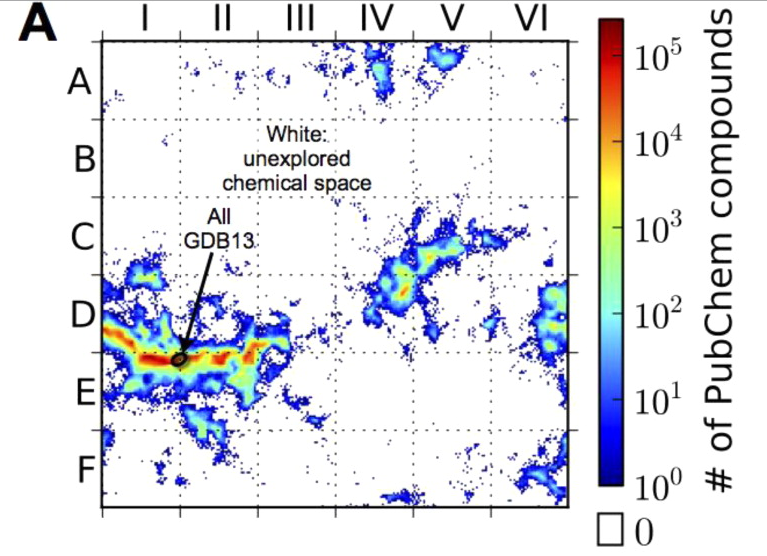
\includegraphics[width=0.9\textwidth]{fig/uncharted_space.png}}
\caption[Unexplored chemical space]{\emph{Stochastic voyages into uncharted chemical space produce a representative library of all possible drug-like compounds} \DUrole{cite}{Virshup2013}.}
\end{figure}

Figure 1.1 shows that along the first two axes of the principal component analysis of that 40-dimensional chemical space  reveals a map is mostly blank, which means that, despite having synthesized more than 100 million compounds, scientists have been focusing on the same regions over and over (an so has nature). For example, the GDB13 database, an enumerated library of compounds under 13 atoms which is the largest database of chemical structures currently available, only accounts for a strikingly-low 0.07\% of the self-organizing map representation of the SMU. This could suggest that if new molecular design approaches are established, new regions could be visited and \emph{brought to life}.


%___________________________________________________________________________

\section*{\phantomsection%
  1.2. Chemobiology and the chemobiological space%
  \addcontentsline{toc}{section}{1.2. Chemobiology and the chemobiological space}%
  \label{chemobiology-and-the-chemobiological-space}%
}

Creating new molecules and biomolecules stands on a series of physicochemical considerations that include different forms of interactions:
%
\begin{quote}
%
\begin{itemize}

\item Covalent interactions. The creation of new strong bonds between atoms.

\item Coordination interactions. The use of metal and transition metals.

\item Non-bonding interactions. Van der Waals, dispersive forces, hydrogen bonds, polar interactions.

\end{itemize}

\end{quote}

Chemobiological developments combine all the afore mentioned interactions in a hybrid system that merges chemical compounds and biological moieties in a functional entity, such as in artificial enzymes, biosensors, biomarkers or supra(bio) molecular complexes. The creation of these systems result in a very high dimensionality which existent strategies cannot face easily: all three chemical, biological and conformational axes need to be explored at once (a simplified graphical representation can be seen on figure 1.2).
%
\begin{quote}
%
\begin{itemize}

\item The \textbf{conformational axis} holds all the possible geometric operations that a set of atoms can experiment, such as global translation and rotation or local torsion, rocking and bouncing. This kind of changes can make structures stable, unstable or metastable.

\item The \textbf{chemical axis} refers to the addition and removal of atoms in a molecule, as well as specific substitution of its functional groups.

\item The \textbf{biological axis} explains residue mutations, and travelling all along the sequence of the species; mainly in its active regions.

\end{itemize}

\end{quote}
\begin{figure}
\noindent\makebox[\textwidth][c]{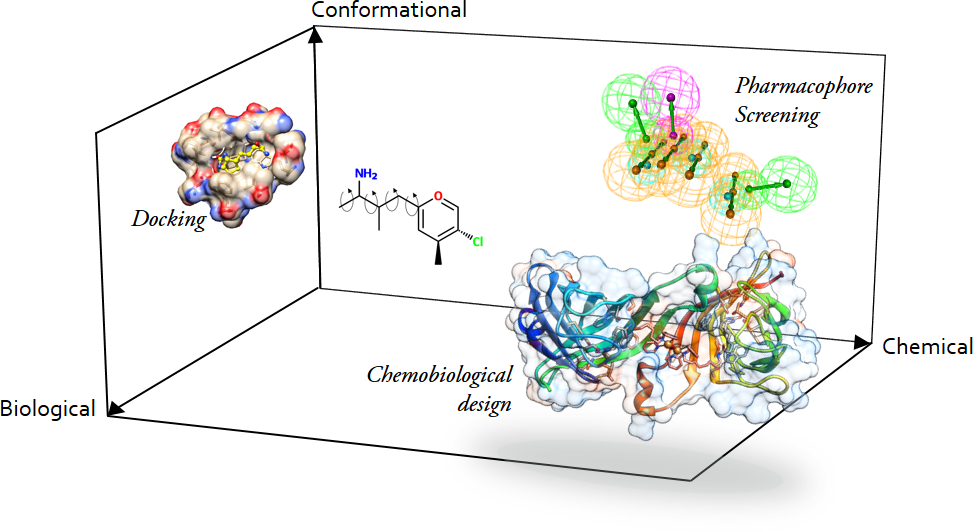
\includegraphics[width=\textwidth]{fig/3d_space.png}}
\caption[A highly dimensional search space]{The chemobiological space of hybrid chemobiological essays can be studied in terms of three main axes: conformational, chemical and biological variations.}
\end{figure}

One could argue that the chemical and biological axes are redundant --- after all, biological structures are all about chemistry and, in fact, biological variations can be considered as a functional abstraction of a subset of the chemical space. However, biological modifications are treated separately because the nature of these changes are well described from the biochemical point of view; i.e., a mutation in a given residue can disrupt the structure of an alpha-helix, or a crucial disulfide bond could be broken.

To grasp an idea of the size of this highly dimensional space, we can think of standard docking essays. Although they only explore the conformational axis, they already require a simplified expression of binding energies to help face their search space. On its part, pharmacophore studies add some details from the chemical plane, but they do not handle a lot of biological variations. How could we even think of handling all the three axes simultaneously?

The real situation is even more complex, though. To take full advantage of these hybrid approaches, biotechnologists tend to make use of exotic organometallic centres that bring new kinds of reactivity to the table, as well as heavily modified aminoacids that generate novel structural scaffolds in a biocompatible environment, drastically enlarging the search space. All of this poses a challenge that demands novel strategies which allow explosive exploration of a hypervolume whose size does not allow an accurate representation. In fact, at the moment, both experimental and theoretical communities lack tools that would allow them to even start sketching initial molecular scaffolds.


%___________________________________________________________________________

\section*{\phantomsection%
  1.3. In silico strategies for molecular design%
  \addcontentsline{toc}{section}{1.3. In silico strategies for molecular design}%
  \label{in-silico-strategies-for-molecular-design}%
}

Being able to test if a candidate molecular sketch is an acceptable solution for a given problem without the need of actually synthesizing it is an invaluable asset. Thus, it is not surprising that computer-assisted molecular design (CAMD) is becoming an increasingly demanded area in the field \DUrole{cite}{Hoffer2013,Tang2014,Hoksza2014}. While CAMD have been proved successful in a decent amount of cases \DUrole{cite}{Clark2006,Kubinyi2009}, most extended methods still suffer from the same diversity issues found in combinatorial chemistry, especially when it comes to hybrid disciplines that extend beyond traditional drug design, such as chemobiology.

\subsection*{\phantomsection%
  1.3.1. Available strategies%
  \addcontentsline{toc}{subsection}{1.3.1. Available strategies}%
  \label{tree-ordering-and-statistical-analysis}%
}

Different strategies have been applied with more or less success in molecular design. While the search space can be huge, it is also discrete. With this in mind, some attempts have gone for exhaustive enumeration, in which a part of the search space is explored sequentially. Though it may seem inefficient, it has produced relevant results in some cases, as proved by \DUrole{citein}{Fink2007}.

Exhaustive enumeration can work well if the constraints are limiting enough to reduce the search space to a feasible portion, but with bigger problems it is no longer the case. One alternative is to classify the enumerated elements in branches so, if the elements of one branch are detected as fruitless, they can be removed at once by pruning that branch. These algorithms are called \emph{Branch and Bound} (BB) and have been implemented successfully in several fragment-based drug designs \DUrole{cite}{Hajduk2007}.

However, the applicability of BB is limited and in some cases stochastic techniques are very much preferred, such as Monte Carlo-like algorithms (MC) \DUrole{cite}{Das2008}, or even evolutionary approaches (EA) --- particularly, genetic algorithms (GA). This former group of strategies are extensively used in docking programs, like GOLD \DUrole{cite}{Jones1997} or AutoDock \DUrole{cite}{Trott2010}. Evolutionary algorithms are a common choice because they deal with several candidate solutions at once, which is also the case in these multi-objective optimization problems. This common partnership will be further detailed in chapter 3.

A recent advance proposes a new paradigm that focus on inverse relationships. Instead of enumerating a series of ligands and testing their fitness to the problem, inverse molecular design rely on optimizing molecular property functionals with respect to a limited number of chosen variables \DUrole{cite}{Huggins2009}.

\subsection*{\phantomsection%
  1.3.2. The focus of commercial platforms%
  \addcontentsline{toc}{subsection}{1.3.2. The focus of commercial platforms}%
  \label{protein-ligand-docking-and-virtual-screening}%
}

To date, computational strategies in molecular design only focus on reduced dimensions of the chemobiological space. Although the number of available molecular design programs is not little by any means, zero to none can be actually used to deal with all the variables that are relevant to generate chemobiological hybrids. Not even for a mere sketch. Indeed, most are concentrating on aspects related to protein engineering and drug discovery. With the increase of the quality of molecular modelling tools, many commercial packages now offer platform towards both fields --- i.e., Schrodinger LLC offers several commercial packages that could help in these new challenges, such as Biologics Suite or Small-Molecule Drug Discovery Suite \DUrole{cite}{schrodinger}, as well as Accelrys' Materials Studio and Discovery Studio, now part of 3DS' Biovia \DUrole{cite}{accelrys}. 

Freeware projects usually focus on a single application with a less versatile approach that requires custom scripting for more complex projects. Commercial packages do allow more integrative experiments, though their licenses usually have an astronomical price tag, even for the academia. Nonetheless, they can be considered as the reference in the field and offer a sneak peek of the state of the art in that area. Those programs generally focus on simulating three majors, following developed:


%___________________________________________________________________________

\subsubsection*{\phantomsection%
  1.3.2.1. Protein-ligand docking and virtual screening%
  \addcontentsline{toc}{subsubsection}{1.3.2.1. Protein-ligand docking and virtual screening}%
  \label{protein-ligand-docking-and-virtual-screening}%
}

Existing computational procedures used in potein-ligand dockings are dedicated to finding a suitable spatial accommodation of a small ligand inside a protein pocket. This is mainly a conformational problem that is not really aimed at the exploration of the chemical space or the biological space (axis X and Y, figure 1.2). Fully visiting both axes at once is not very common, and if they even do it, existing solutions tend to only consider small slices of that additional dimension. These extra detours are usually performed with a second set of calculations like in virtual screening or approaches based on library search, thus starting with an already biased subspace that could have neglected some good candidates for this second stage.


%___________________________________________________________________________

\subsubsection*{\phantomsection%
  1.3.2.2. Conformational exploring%
  \addcontentsline{toc}{subsubsection}{1.3.2.2. Conformational exploring}%
  \label{conformational-exploring}%
}

The programs mentioned before also feature conformational exploration engines. For example, Schrodinger's Small-Molecule Drug Discovery Suite and Biologics Suite rely on advanced molecular mechanics and molecular dynamics, with implicit or explicit solvents, both for small molecules and macromolecular systems. Accelrys' proposal also rely on molecular dynamics simulations using CHARMm and a GB solvent model. Alternative solutions include the use of Monte Carlo coarse-grain models, such as CABS \DUrole{cite}{Jamroz2013}, or model normal mode-based approaches, such as NMSim \DUrole{cite}{Ahmed2011}.


%___________________________________________________________________________

\subsubsection*{\phantomsection%
  1.3.2.3. Enzyme design%
  \addcontentsline{toc}{subsubsection}{1.3.2.3. Enzyme design}%
  \label{enzyme-design}%
}

Commercial packages now offer bioengineering tools that allow, at most, seeing the effect of a few mutations on the physicochemical properties of the system or the implications on their natural ligand recognition processes, but not for design. Designing an enzyme from scratch is still far from our current possibilities. It would mean being able to accurately predict the folding of a given sequence of residues, one of the main unsolved problems in biochemistry. As of today, scientists have to be content with optimizing already existing proteins. The technique involves screening a protein database to find an adequate starting point and the optimize its active site to allocate a given transition metal through a series of directed evolution cycles. As of today, David Baker \DUrole{cite}{Khersonsky2011,Althoff2012} and Stephen L. Mayo \DUrole{cite}{Privett2012} have been successful at it by using slightly different approaches. These two examples prove that CAMD can actually help in the design of new enzymes, but they also point that the technique is still in development and that several experimental steps are still needed.


%___________________________________________________________________________

\section*{\phantomsection%
  1.4. Limitations of nowadays tools for biochemical design%
  \addcontentsline{toc}{section}{1.4. Limitations of nowadays tools for biochemical design}%
  \label{limitations-of-nowadays-tools-for-biochemical-design}%
}

The building of some artificial chemobiological entities can be described as a complex docking problem where, in addition to standard non-bonded interactions, bonded, covalent interaction as well as combinatorial considerations are necessary. Such aspects are out of the scope of standard molecular modelling tools: while molecular design is closely linked to covalent bonding and metal coordination, a marginally considered aspect in most cases. The following sections will discuss the different limitations found nowadays.


%___________________________________________________________________________

\subsection*{\phantomsection%
  1.4.1 Covalent bonds%
  \addcontentsline{toc}{subsection}{1.4.1 Covalent bonds}%
  \label{covalent-bonds}%
}

Of all the available docking programs, only a few support covalent docking essays. GOLD and, more recently Glide's CovDock \DUrole{cite}{ToledoWarshaviak2014} do provide an option to anchor the ligand to one of the protein atoms, and so does AutoDock, but that's it. If a researcher wanted to try several anchoring points in a branched ligand, he or she would have to mimic all the covalent bonds sequentially, one bond at a time. Let alone looking for possible hydrogen bridges or hydrophobic patches for a given set of atoms at the same time.

Though alternative methods are available, they are not versatile enough to meet our requirements, or rely on modifications on existent programs that tend to be overly complicated \DUrole{cite}{Katritch2007}. A promising new option called CovalentDock was released past year as a modification of the popular AutoDock. This novel program implements a new layer in AutoGrid to help screen the possible acceptors and donors in the protein and the ligand, which results in improved accuracy \DUrole{cite}{Ouyang2013}. However, those programs are purely aimed at dealing with one or two covalent bonds at the most in order to reproduce the mechanism of the few covalent drugs (i.e., AZT). Nothing exists to deal with a random and automatic generation of multiple covalent bonds like those necessary for the design of hybrid biochemical systems, such as small peptides or artificial enzymes.


%___________________________________________________________________________

\subsection*{\phantomsection%
  1.4.2 Metal and coordination bonds%
  \addcontentsline{toc}{subsection}{1.4.2 Metal and coordination bonds}%
  \label{metal-and-coordination-bonds}%
}

GOLD or Glide are docking programs that support metal moieties in the protein but cannot predict how metals --- naked or embedded --- behave in wider systems like organometallic molecules or nanoparticles. Though some attempts have been successful at extending this limitation with a series of tricks, such as substituting the metal elements with dummy atoms, these \emph{hacks} force to consider the first coordination sphere of the metal as a rigid shell \DUrole{cite}{Ortega-Carrasco2014}.

FlexX is another docking program that includes a knowledge-based approach to handle ligands with metallic centres and is able to predict coordination geometries, using that information as part of the docking process \DUrole{cite}{Seebeck2008}. However, one of the challenges in building chemobiological hybrids is using exotic transition metals as an instrumental part of the reactivity.


%___________________________________________________________________________

\subsection*{\phantomsection%
  1.4.3 Conformational exploration of the chemobiological space%
  \addcontentsline{toc}{subsection}{1.4.3 Conformational exploration of the chemobiological space}%
  \label{conformational-exploration-of-the-chemobiological-space}%
}

Dealing with conformational, chemical and biological changes to travel in the chemobiological space is one of the grails in molecular modelling. Nowadays, most docking strategies consider almost of degrees of freedom of the ligand with the still challenging problem of cyclic systems. Moreover, the majority is able to consider some amount of conformational changes of the protein whether local (by including discrete displacement of the amino acids geometries; i.e., rotamers) or global (i.e., normal modes or molecular dynamics).

Actual mutation of protein residues are not that extended in most used software, since the consequences of such a vast change cannot be easily anticipated. Instead, current approaches resort to experimental techniques like directed mutagenesis to generate different protein scaffolds and then feed the program in use with the resulting crystallographic structures.

With respect to the space concerning the ligand, if the problem is simple enough to not require dynamical building, just conformational variations, one could try using a docking protocol, but the researcher would soon find that most of the programs do not support metal ions at all or, if they do, he or she would face awful complications \DUrole{cite}{Ortega-Carrasco2014}. If it does require dynamical construction, i.e., the ligand itself is not given and only a few building blocks and a couple of constraints are given, there is not a single piece of software that can even provide a few tentative sketches of the solutions.


%___________________________________________________________________________

\section*{\phantomsection%
  1.5. Designing novel chemobiological hybrids: the search for an initial sketch%
  \addcontentsline{toc}{section}{1.5. Designing novel chemobiological hybrids: the search for an initial sketch}%
  \label{designing-novel-chemobiological-hybrids-the-search-for-an-initial-sketch}%
}

An example of the most promising fields in chemobiological design is the creation of artificial enzymes that combine well-known biological scaffolds with established industrial catalyst systems, which usually include transition metal centres, thus allowing exotic chemical activities to take place in a biocompatible environment.

As discussed, working on these systems with existent solutions forces the researcher to push the boundaries of the programs to untested situations, usually resorting to workarounds for which the software were not designed to. Avoiding dirty tricks like these and providing a straight-forward platform that can cope with these experiments out of the box are some of the main motivations behind this dissertation. Thus, our objective is to provide a molecular-sketching platform that can deal with all these problems by delivering an easy-to-deploy interface that can respond to commonly asked questions in the molecular design world.

\chapter{Objectives}

The current state of the art in molecular design software shows that available programs are very good at handling certain search spaces, but cannot face the complexities that arise from combining some of them. Some of them would take too long to give back an answer, while others would lack the means to provide a reasonable way to do it without hacking some parts of it.

In response to the demands of the chemobiological design community, a new tool was designed to help address these issues. The results of my Masters in Science has been named after the famous Catalonian architect, Antoni Gaudí. \textbf{GAUDI} stands for \textbf{G}enetic \textbf{A}lgorithms for \textbf{U}niversal \textbf{D}esign \textbf{I}nference. It consists of a novel platform that aims to satisfy a increasingly demanding area in molecular design: artificial chemobiological systems. It does so by providing the researchers with a powerful multi-objective optimization engine to explore the huge search space that chemobiological design problems usually present.

In order to demonstrate the strengths of GAUDI, a complex artificial system designed by Thomas Ward was chosen. This artificial hemocyanin uses a streptavidin-biotin scaffold to support an oxygen-binding di-copper centre. The system made for a solid challenge since it simultaneously demanded to solve a docking problem, handling a transition metal and designing an adequate set of linkers. This required to develop several modules from scratch, such a dynamical molecule builder, a graphic user interface or a Van-der-Waals screening engine.

In fact, during the implementation process of our approach, we realised that it was versatile enough to deal with other kind of experiments, too. We could not resist and tried to apply our gained savoir-faire to an additional essay. As a result, chapter 05 shows the extensibility of GAUDI in action by performing a refinement essay of a GRID-minimized experiment. This former case study demonstrates that GAUDI can work just fine with both top-down and bottom-up approaches.

As a result, the main objectives of this dissertation are:
%
\begin{itemize}

\item Designing a multi-objective genetic optimization engine that can face exploring a huge multidimensional space.

\item Implement a lightweight GUI viewer that can help examine thousands of chemically and physically sound solutions.

\item Solve an artificial enzyme design problem by proposing several candidate structures, as discussed in chapter 4.

\item Apply inverse molecular design by optimizing the coordination sphere of an aluminium centre in a series of possible protein binders, as discussed in chapter 5.

\end{itemize}



\chapter{Introducing GAUDI\textsubscript{ASM}}
%_________________________________________________________________

\section*{\phantomsection%
  3.1. What is GAUDI\textsubscript{ASM}%
  \addcontentsline{toc}{section}{3.1. What is GAUDIASM}%
  \label{what-is-gaudiasm}%
}

Chemobiological researches are often challenged with molecular design tasks that combine several types of compounds, proceeding from  biological to chemical environments, including organic and inorganic structures. These hybrid systems are, by far, much less studied than their individual parts, which results in an obvious lack of software tools that can help to confront the challenges they propose. For example, we can easily find conformational explorers like Confab \DUrole{cite}{OBoyle2011} or Balloon \DUrole{cite}{Vainio2007}, but they just focus on a single axis of the multidimensional space that must be explored. A fresh approach is needed, and that is the blank GAUDI\textsubscript{ASM} will try to fill.

\textbf{GAUDI}\textsubscript{ASM} stands for \textbf{G}enetic \textbf{A}lgorithms for \textbf{U}niversal \textbf{D}esign \textbf{I}nference and \textbf{A}tomic \textbf{S}cale \textbf{M}odelling. It consists of a novel platform that aims to satisfy an increasingly demanding area in molecular design: artificial chemobiological systems. It does so by providing the researchers with a powerful multi-objective optimization engine to simultaneously explore all the variables (the three axes exposed in the introduction on figure 1.2) that compose the huge search space chemobiological design problems usually present. Given a customizable list of objectives, GAUDI\textsubscript{ASM} will optimize the given compounds to simultaneously satisfy all the requested criteria.


%___________________________________________________________________________

\section*{\phantomsection%
  3.2. The methodology: Genetic exploration with multi-objective capabilities%
  \addcontentsline{toc}{section}{3.2. The methodology: Genetic exploration with multi-objective capabilities}%
  \label{the-methodology-genetic-exploration-with-multi-objective-capabilities}%
}

Most real-life optimization problems comprise several (usually conflicting) objectives, but they tend to focus on just one of them, describing the remaining ones as restraints \DUrole{cite}{Konak2006}. If we were to buy a car with the most powerful engine but also the most environmental friendly, and the cheapest possible price, we would probably set a maximum price and then decide on an acceptable compromise between power and eco-friendliness. However, this kind of strategy is not really solving the optimization problem, since it starts by discarding a portion of the search space; i.e., setting a restraint on the price\footnote{Objectives and restraints may seem to refer to the same concept, but during this dissertation a slight difference will be made. While objectives are treated independently of other decision variables, restraints are not. Objectives rule the calculations and are assisted by the limits imposed by the restraint. This doesn't happen the other way around: a variable expressed as a restraint will not worsen the situation of a variable expressed as an objective because the experiment has been designed to satisfy the requirements of the so-called objective.}.

Molecular design are multi-objective optimization problems, but they are not usually treated as such. Most of the existent approaches consist of an energy minimization or other conformational exploration processes guided by a set of user-provided restraints. As a result, this strategy provide a solution under a very restrictive combinatorial space and may be leaving a lot of the possible solutions out of scope. Why would we want to renounce to any chances of finding the right molecular construction that will solve our problem?

Having multiple objectives implies that the concept of a single \emph{optimum} solution is no longer valid. Instead, multi-objective optimization algorithms usually propose a set of good \emph{trade-offs} between the  variables to consider \DUrole{cite}{Coello2007}. This idea is known as \emph{Pareto optimality}, as enunciated by Wilfredo Pareto in his studies of income distribution.

Given a set of candidate solutions, a Pareto improvement is a change that can make at least one solution better off, without worsening the situation of the other candidate solutions. When no further Pareto improvements can be applied on the set, that set is said to be \emph{Pareto optimal}. The so-called \emph{Pareto front} is the set of all the Pareto optimal solutions, and, in principle, all of them are good answers to the problem. With \texttt{n} dimensions or objectives, the Pareto front can be depicted as a hypersurface that hosts the optimal solutions of the hypervolume\footnote{While hypervolume refers to a n-dimensional space (more than three dimensions), hypersurface refers to the a reduced (n-1)-dimensional version of that space.}.

Finding the true Pareto front can be difficult, but it can be approximated by a rich set of non-dominated solutions. A solution \texttt{a} is set to dominate solution \texttt{b} if it solves at least one of the objectives better than \texttt{b}, without losing to \texttt{b} in any of the remaining objectives \DUrole{cite}{Deb1999}. \texttt{a} dominates \texttt{b} if it makes for a better answer to the problem; in other words, non-dominated solutions are closer to the solution than dominated ones. Dominance is one of the key aspects of multi-objective optimization, and is used extensively in well-known algorithms such as NSGA-II \DUrole{cite}{Deb2002}.

Using multi-objective optimization algorithms allows us to efficiently examine all the decision variables at once, avoiding the design of sequential workflows that work on a single aspect at a time. For example, instead of optimizing the length and mass of the compound, then looking for appropriate chemical substitutions and finally finding the proper orientation inside the binding pocket of the protein, we can just enter all the parameters into the input and let the optimization process do its work. It is not only more comfortable for the user, but also more efficient and exhaustive, since it avoids losing candidate solutions that could have been welcome in forthcoming stages of the optimization.


%___________________________________________________________________________

\subsection*{\phantomsection%
  3.2.1. Dealing with several solutions at once%
  \addcontentsline{toc}{subsection}{3.2.1. Dealing with several solutions at once}%
  \label{dealing-with-several-solutions-at-once}%
}

As using Pareto optimality criteria usually means working with multiple solutions, it makes sense to use exploration algorithms that can deal with several candidate solutions at once. One of the most common choices is to use genetic algorithms (GA). GAs are part of evolutionary algorithms, which, as their name states, are heavily inspired by Darwin's evolution theory. In fact, they take a lot of the nomenclature from it. For example, a candidate solution is called \emph{individual}, whose terms, variables or parameters are named \emph{genes} or \emph{chromosomes}. The ground idea is to expose the candidate solutions to an evolutionary simulation, in which the fitness of the individuals is determined by an evaluation function that runs the optimization process.

A simple GA starts by generating a random set of \emph{individuals}, the so-called initial \emph{population}. Then, that population is exposed to a series of evolutionary operators, such as gene mutation, chromosome recombination or, in some approaches, migration. As a result, a new set of individuals is produced by the parent population. Some of them will be \emph{fitter} than their preceding counterparts, some of them not. That's why all of them are tested by the evaluation function, which will return their \emph{fitness} in the form of a score. Only the fittest individuals will be allowed to continue in the solutions pool or, in biological terms, \emph{selected} to take part in the next \emph{generation} \DUrole{cite}{Goldberg1989,Mitchell1998}.
\begin{figure}
\noindent\makebox[\textwidth][c]{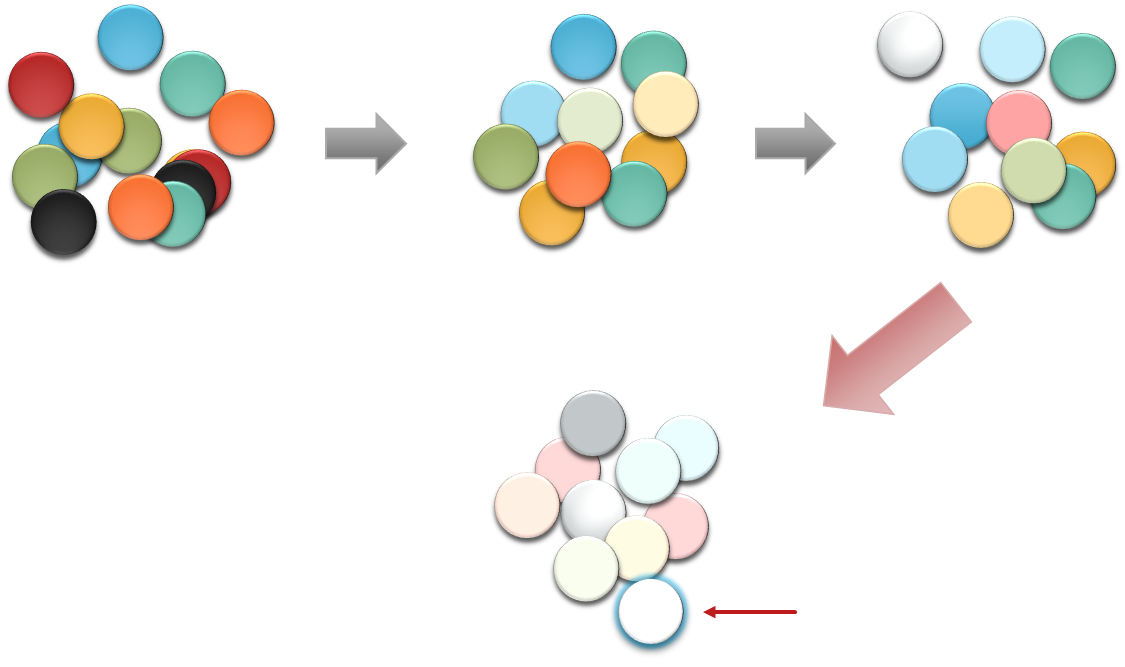
\includegraphics[width=0.9\textwidth]{fig/ga.png}}
\caption[Simulating evolution with Genetic Algorithms]{Genetic Algorithms simulate evolution in a randomly-generated population of possible solutions.
Each generation, the best solutions are selected and allowed to exchange and mutate their terms, thus contributing to improve the overall fitness of the population. After a number of generations, a set of good-enough individuals is usually found. In this example, we are trying to generate a white circle (RGB-coded as 255,255,255) from a population of randomly-coloured circles by maximizing the sum of the colour indices. One of the first consequences of the simulated evolution is the loss of the black circles (RGB-coded as 0,0,0), which do not contribute to getting to the white colour. Soon enough, the results become apparent and the circles begin to show lighter colours. After n generations, the first white circle is found and, after enough iterations, the whole population would be white.
If we needed to assess the radius of the circles too, we would have to rely on a second run of the experiment that started with a biased population of previously-selected circles. With a multi-objective optimization algorithm like the one GAUDI\textsubscript{ASM} uses, this is not a problem, since both axes can be evaluated simultaneously. There is no need for a fabricated weighted sum which would have no meaning since the importance of each parameter is not known beforehand.}
\end{figure}

After a few generations, the population will have evolved towards a reasonable set of solutions that approximate the Pareto optimal front. However, as the number of objectives increases, it becomes harder to accurately reconstruct the true Pareto front. In fact, it can consist of hundreds of solutions. To determine which one the researcher is really looking for, a scalarization technique must be applied --- after all, only a section of the hypersurface might be necessary. Of all the possible approaches, weighted sums are one of the most common due to their simplicity, but also encompasses a few limitations, such as knowing the importance and precedence of the different objectives beforehand \DUrole{cite}{Hwang1979}. As GAUDI\textsubscript{ASM} mixes energetic, geometric and chemobiological criteria together, this cannot be anticipated easily; instead, GAUDI\textsubscript{ASM} returns the whole Pareto front, leaving the decision up to the researcher's own criterion and the visual advice provided by GaudiView, GAUDI's accompanying GUI tool.

%___________________________________________________________________________

\section*{\phantomsection%
  3.3. Main features%
  \addcontentsline{toc}{section}{3.3. Main features}%
  \label{main-features}%
}

GAUDI\textsubscript{ASM} relies on two main projects to achieve its functionality: UCSF Chimera \DUrole{cite}{Chimera} and DEAP \DUrole{cite}{Deap}, both written in Python. On top of these two main pillars, a custom framework during this Master thesis has been implemented to help guide molecular design essays. Further technical details of this implementation are discussed in Appendix A.
\begin{figure}
\noindent\makebox[\textwidth][c]{\includegraphics[width=0.9\textwidth]{fig/pseudo.pdf}}
\caption[GAUDI\textsubscript{ASM} main launcher pseudocode]{Pseudocode of the launcher script that is launched in every GAUDI\textsubscript{ASM} experiment.}
\end{figure}

%___________________________________________________________________________

\subsection*{\phantomsection%
  3.3.1 Molecular design guided by evolutionary pressure%
  \addcontentsline{toc}{subsection}{3.3.1 Molecular design guided by evolutionary pressure}%
  \label{molecular-design-guided-by-evolutionary-pressure}%
}

GAUDI\textsubscript{ASM} features a simple but powerful compoumd design tool that allows wider chemical exploration possibilities with respect to most actual software with similar purposes. Instead of providing a list of already built ligands, the user can input a list of alphabetically-sorted directories that contain individual molecular building blocks. GAUDI\textsubscript{ASM} will then parse the supplied files and build the resulting ligands on the fly, as requested by the genetic algorithm selection operators.

The builder does not impose any restraints on the building blocks, as long as they are formatted as standard mol2 files. By default, the blocks will be joined by the atoms that present the least and greatest serial number, respectively, but the user may specify any other atoms in an additional input.

This approach is versatile enough to explore the solution landscape in terms of spatial requirements (\emph{``How many atoms would I need to build a ligand that can bridge these two subunits?''}) and chemical substitutions (\emph{``Which groups should this ligand of 10 carbons feature so it can form an hydrogen bond with aspartic acid 100?''}). Thanks to the integrated parser, a short list of SMILES strings will suffice to launch an initial essay.

%___________________________________________________________________________

\subsection*{\phantomsection%
  3.3.2 Biochemical and steric optimization of the search space%
  \addcontentsline{toc}{subsection}{3.3.2 Biochemical and steric optimization of the search space}%
  \label{biochemical-and-steric-optimization-of-the-search-space}%
}

GAUDI\textsubscript{ASM} makes full use of Dunbrack's \DUrole{cite}{Dunbrack1994} and Dynameomics \DUrole{cite}{Scouras2011} rotameric libraries to optimize the conformational space of the protein. Just select the desired residues and, if desired, activate a local mutation flag so that the algorithm randomly swaps the selected residue with any other natural amino-acid. This feature enables us to explore the search space in both conformational and biochemical dimensions.

The ligand flexibility is also configurable. Instead of letting choose between \emph{rigid} and \emph{flexible}, the input file requires a maximum torsion angle that will determine the global flexibility. If is set to zero, it will behave as a rigid compound; setting it up to 360 will have the opposite effect. Any integer in between is acceptable, so it is possible to choose a reasonable torsion that will provide just the right amount of flexibility without losing the initial conformational information.

%___________________________________________________________________________

\subsection*{\phantomsection%
  3.3.3 Forcefield-less energetic terms%
  \addcontentsline{toc}{subsection}{3.3.3 Forcefield-less energetic terms}%
  \label{forcefield-less-energetic-terms}%
}

As of now, GAUDI\textsubscript{ASM} relies on four forces that are usually sufficient to guide the exploration in energetic terms. Specifically, it supports hydrogen bonds discovery (based on geometrical criteria, as proposed by \DUrole{citein}{Mills1996}, hydrophobic patches complementarity detection (as expressed by a rough Lennard-Jones-like calculation, see equation A.1) and steric clashes (analytically calculated as overlapping Van der Waals volumes, as proposed by \DUrole{citein}{Eyal2004}; see equation A.2), and solvent accessible and excluded surface areas calculations (based-off MSMS \DUrole{cite}{Sanner1996}). Again, more technical details on these aspects are given in Appendix A.

Artificial systems often take advantage of organometallic groups to produce new chemical reactions in a very precise chemospecific context. Because of the complexity to parametrize metal ions in force fields and the crude approximation of their electronic nature in the scoring functions used in docking programs, standard molecular procedures are rather little adequate for metal containing systems. Since quantum mechanics are still a long way of being used in screening essays, true energetic terms are inevitably left out of scope. To help palliate this issue, GAUDI\textsubscript{ASM} proposes a workaround that exploits the multi-objective capabilities and provides several modules that try to resemble the most featured of metal bioinorganic interactions.

With this simple approach, metals can be happily part of both the protein and the ligand, overcoming one of the main limitations found in most of docking programs, which apparently have been ignoring this field of molecular design. In fact, nothing prevents us from using a metal ion as a ligand and optimize the surrounding rotamers to find a suitable coordination geometry, as it will be discussed in chapter 5.


%___________________________________________________________________________

\subsection*{\phantomsection%
  3.3.4 GaudiView: A GUI explorer for complex sets of candidate solutions%
  \addcontentsline{toc}{subsection}{3.3.4 GaudiView: A GUI explorer for complex sets of candidate solutions}%
  \label{gaudiview-a-gui-explorer-for-complex-sets-of-candidate-solutions}%
}

As previously stated, multi-objective optimization processes often generate more than one possible solution to the problem. To help find the most suitable ones, the results of this thesis also includes a visual tool to help explore the Pareto Front produced GAUDI\textsubscript{ASM}: GaudiView. GaudiView has been tailored as a native Chimera extension that lazy-loads the whole range of solutions, no matter the size. Some complex experiment can produce thousands of candidate individuals, so the program must be both efficient and effective. Lazy-loading avoids long initial wait times, since the file is only loaded into memory when it's actually requested. This is the same approach that GAUDI\textsubscript{ASM} internally uses to build the ligands library on the fly.

Furthermore, the GUI tool includes multiple sorting and filtering utilities to help discern the adequate portion of the Pareto hypersurface. In some complex cases, the set of solutions may not include what the researcher would call a \emph{perfect solution}, but he or she may be able to identify a \emph{pretty good one} if some trade-offs are applied. Instead of performing another run, GaudiView allows to parse the whole Pareto front and retrieve the most promising results effortlessly.

Last but not least, a number of goodies have been included to add special visual support in some specific cases. GaudiView is able to provide effective integration channels with some powerful built-in tools of UCSF Chimera, such as the Metal Geometry utility or the MMTK minimizer. This premium features open the doors to a vertical integrative platform where the researcher would be able to obtain reasonably sound solutions by simply writing a list of objectives.
\begin{figure}
\noindent\makebox[\textwidth][c]{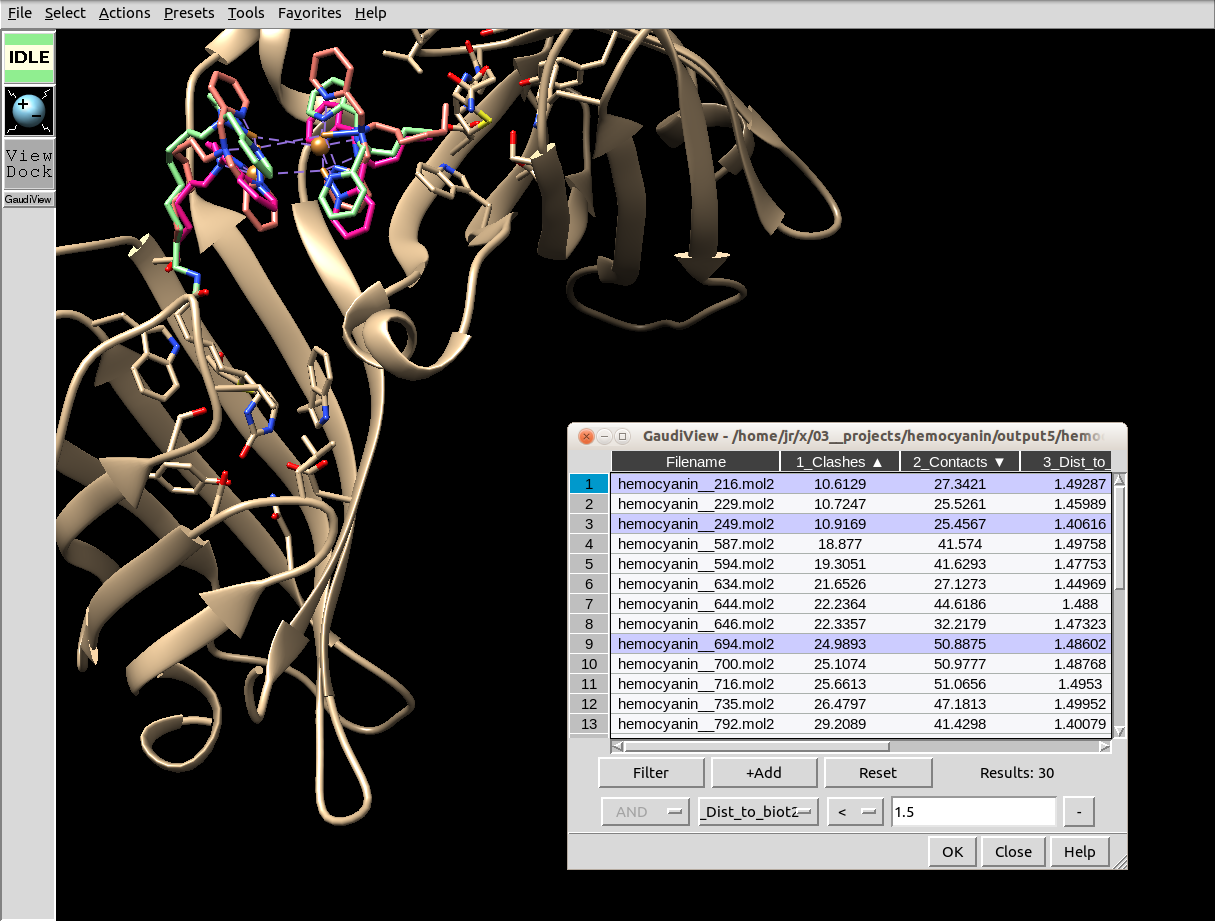
\includegraphics[width=0.9\textwidth]{fig/gaudiview_gui.png}}
\caption[GaudiView, A GUI explorer for complex sets of candidate solution]{GaudiView is a graphic user interface that helps explore the Pareto front of candidate solutions. It features multi-sorting and multi-filtering capabilities and can handle thousands of files thanks to a lazy-loading implementation that drastically reduces the needed amount of RAM.}
\end{figure}

\chapter{Case Study I: Hemocyanin}%



%___________________________________________________________________________

\section*{\phantomsection%
  4.1. Enzymes and organometallics%
  \addcontentsline{toc}{section}{4.1. Enzymes and organometallics}%
  \label{enzymes-and-organometallics}%
}

Life can be seen as a beautifully orchestrated succession of chemical reactions. Most of those reactions could not take place outside cells or, if they did, they would take an unaffordable amount of time. So, how do cells manage to do that? The answer lies in enzymes.

Enzymes are cell-tailored catalysts that provide the necessary environment for biological reactions to take place. The enzymes we know are the product of millions of years of evolution. During that period of time, nature has been sculpting their structure and functionality, so that they become better and better at doing their job. This results in a very specific chemospatial context that greatly lowers the energetic barrier of the transition state, allowing the reaction to happen at mild conditions in a very short period of time.

To fulfil their role, most enzymes do not transform the substrate on their own. Instead, they are helped by a variable number of small diverse molecules called cofactors. One of the more interesting types of cofactors are transition metal compounds. Transition metals exhibit unique chemical properties due to their versatile electronic features which allows them to present a wide range of oxidation states and mechanistic routes absent from purely organic systems.

Artificial metalloenzymes seek to combine the specificity of enzymatic biocatalysts with the reaction possibilities of organometallic groups in a single functional entity. Designing one of these hybrids systems from scratch is still far from being doable, but meanwhile some other less ambitious approaches have been reported successful, such as DNA-based catalysts \DUrole{cite}{Roelfes2005} and several types of protein-based designs. In this former group, three main strategies can be detailed, based on the type of ligand anchoring: dative, covalent or supramolecular \DUrole{cite}{Steinreiber2008}.

\textbf{Dative anchoring} (fig. 4.1.A) features a chelation bond between the metal and some protein residues to ensure the localization of the inorganic moiety in the protein cavity. \textbf{Covalent anchoring} (fig. 4.1.B) consists of covalently binding the cofactor to the protein active site using a reactive residue, such as serine or cysteine. \textbf{Supramolecular anchoring} (fig. 4.1.C) takes advantage of strong non-covalent interactions between the protein receptor and its natural ligands, to which the organometallic catalyst will be covalently attached.
\begin{figure}
\noindent\makebox[\textwidth][c]{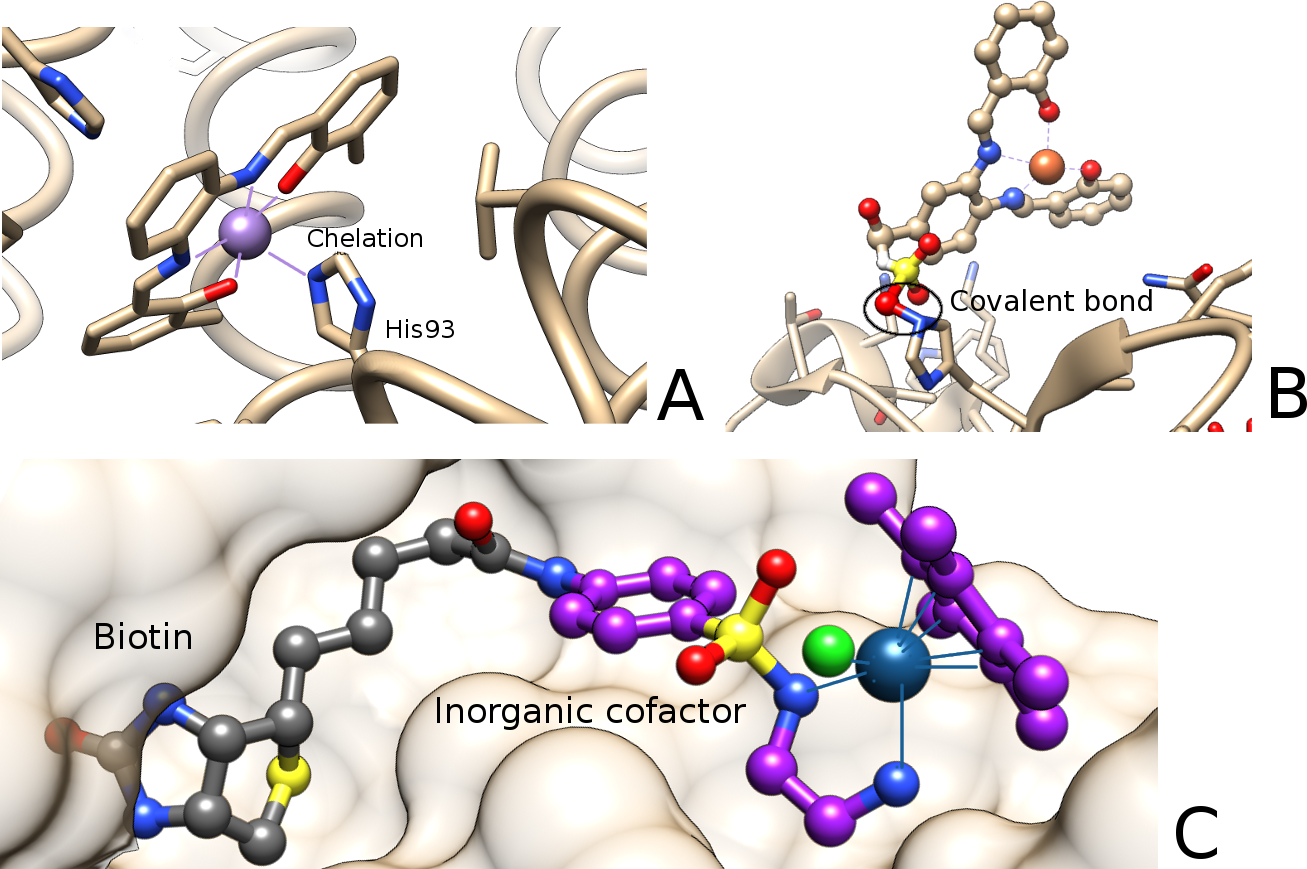
\includegraphics[width=0.9\textwidth]{/home/jr/x/thesis/contents/fig/artificial_types.png}}
\caption[Artificial enzymes design strategies]{\textbf{Main strategies used in protein-based artificial metalloenzymes}. (A) X-ray structure of an artificial metalloprotein obtained by Watanabe and coworkers (PDB code: \texttt{1V9Q}, \DUrole{citein}{Ueno2005}). (B) Fiction model of an artificial system that uses a covalent anchoring strategy. (C) Artificial hydrogenase obtained by Ward and coworkers, which uses an extended biotin as an anchor to insert the inorganic cofactor inside the streptavidin (PDB code: \texttt{3PK2}, \DUrole{citein}{Ward2011}).}
\end{figure}


%___________________________________________________________________________

\subsection*{\phantomsection%
  4.1.1 Streptavidin-biotin technology%
  \addcontentsline{toc}{subsection}{4.1.1 Streptavidin-biotin technology}%
  \label{streptavidin-biotin-technology}%
}

Biotin --- also known as vitamin B7 or H --- is the natural ligand of (strept)avidin, and they both make for a well-known couple in biology due to manifesting the strongest non-covalent interaction in nature: the dissociation constant gets up to $K_d \approx 10^{-14}M$ \DUrole{cite}{Green1975}. The complex is also greatly resistant to extreme pH and temperature levels, organic solvents, proteolytic enzymes and other adverse conditions. All of these features make the system an excellent candidate for supramolecular anchoring techniques and biotechnological developments. So far, this has been one of the most successful strategies in the field.
\begin{figure}
\noindent\makebox[\textwidth][c]{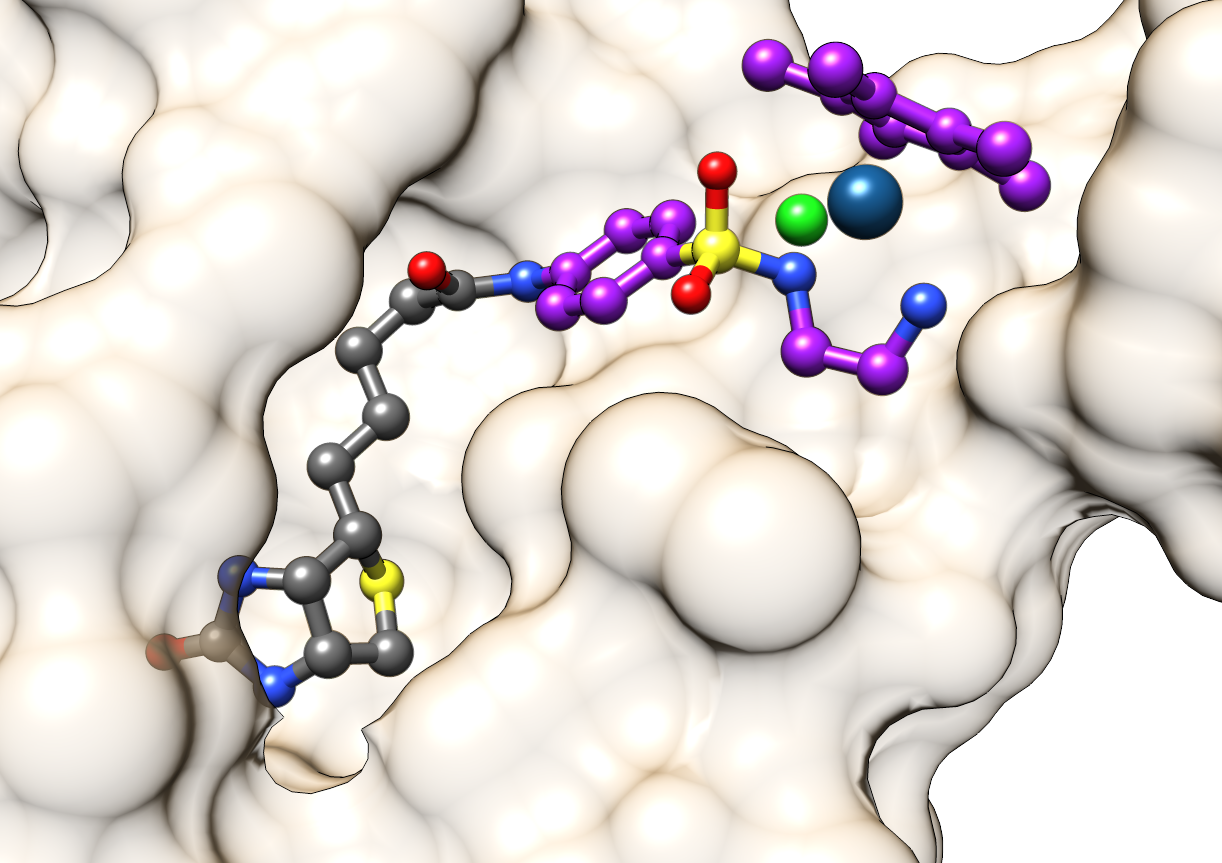
\includegraphics[width=0.9\textwidth]{/home/jr/x/thesis/contents/fig/3pk2.png}}
\caption[Streptavidin-biotin-based artificial hydrogenase]{\textbf{Streptavidin-biotin-based artificial hydrogenase}. Ward et al. are actively working on streptavidin-biotin based systems to implement diverse metallogroups. One of their results is an artificial hydrogenase (PDB: \texttt{3PK2}, \DUrole{citein}{Ward2011}), in which a catalyst (violet dye) is covalently linked to a biotin (grey dye) inside the streptavidin pocket (brown surface). This way, the biotin acts as an anchor that helps place the catalyst inside the streptavidin scaffold.}
\end{figure}


%___________________________________________________________________________

\subsection*{\phantomsection%
  4.1.2 Oxygen transport in invertebrates: hemocyanins%
  \addcontentsline{toc}{subsection}{4.1.2 Oxygen transport in invertebrates: hemocyanins}%
  \label{oxygen-transport-in-invertebrates-hemocyanins}%
}

Hemocyanins are oxygen-carrier proteins that can be found in some invertebrate animals, such as snails, crabs, lobsters or spiders. The transport is achieved thanks to two copper atoms that reversibly bind an oxygen molecule. Oxygen-binding capabilities of copper often result in comparisons with biological iron, though some differences exist. For example, iron is usually found in tetrapyrrole coordinated compounds, while copper prefers imine-nitrogen atoms. In the case of hemocyanin, its two copper atomss coordinate to three histidines each, favouring the dioxygen binding in an global singlet electronic configuration (see figure 4.3).
\begin{figure}
\noindent\makebox[\textwidth][c]{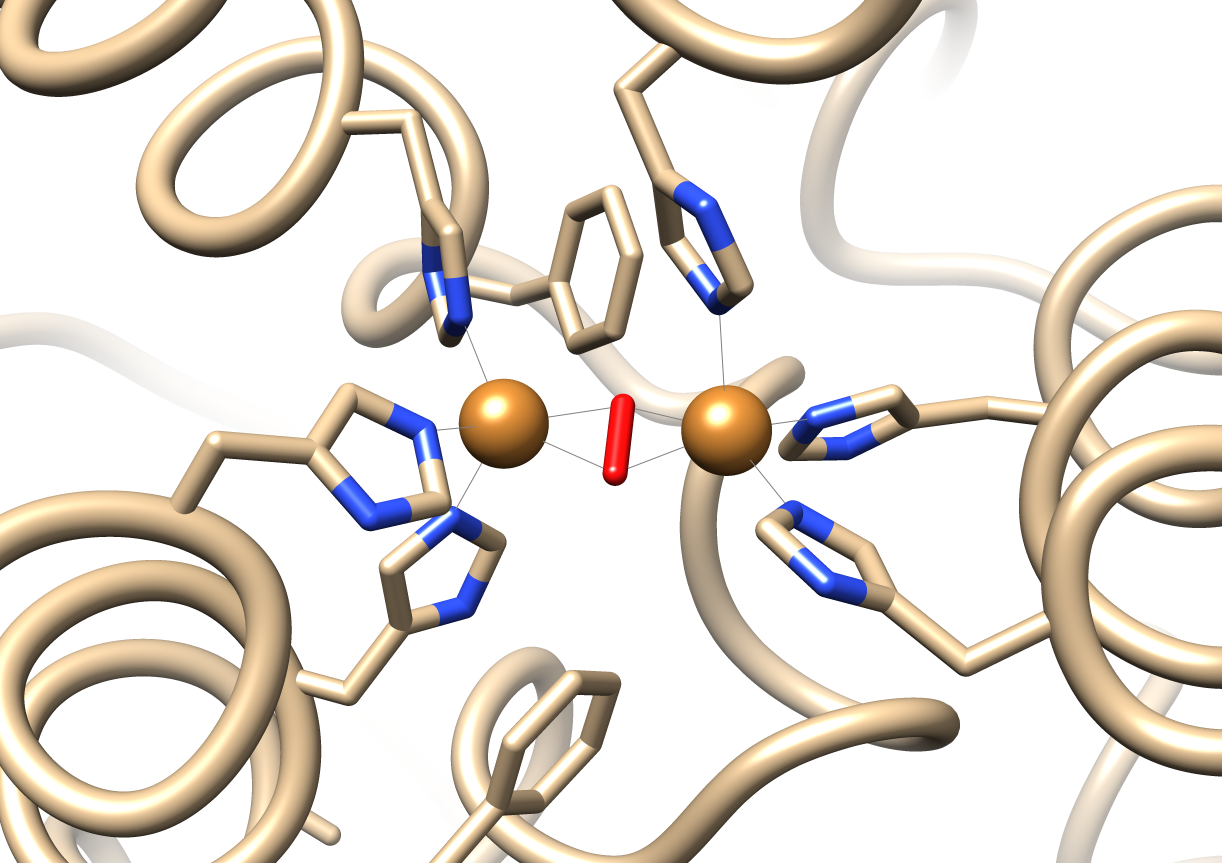
\includegraphics[width=0.9\textwidth]{/home/jr/x/thesis/contents/fig/1nol.png}}
\caption[Oxygenated form of Limulus polyphemus' hemocyanin]{Oxygenated form of \emph{Limulus polyphemus}' hemocyanin. Hemocyanin features a histidine-coordinated di-copper centre that reversibly binds a single molecule of oxygen. (PDB: \texttt{1NOL}, \DUrole{citein}{Hazes1993}).}
\end{figure}
\begin{figure}
\noindent\makebox[\textwidth][c]{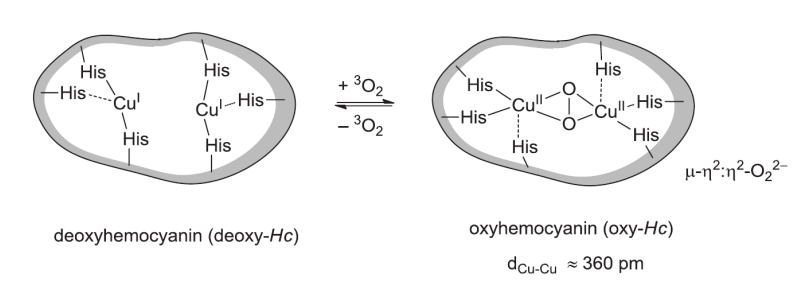
\includegraphics[width=0.9\textwidth]{/home/jr/x/thesis/contents/fig/hemocyanin_schem_kiam.png}}
\caption[Oxidation reaction of the dicopper centre in hemocyanin]{Oxidation reaction of the dicopper centre in hemocyanin. Taken from \DUrole{citein}{Kaim2013}.}
\end{figure}


%___________________________________________________________________________

\section*{\phantomsection%
  4.2. The challenge: an artificial hemocyanin%
  \addcontentsline{toc}{section}{4.2. The challenge: an artificial hemocyanin}%
  \label{the-challenge-an-artificial-hemocyanin}%
}

One of the new experiments Ward's group is working in is an artificial hemocyanin, built upon the streptavidin-biotin system in which the imine-nitrogen atoms are supplied by the biotin-anchored linkers. Several wet-lab attempts have been tried, but none of them have succeeded --- it may be due to unexpected hydrophobic interactions between the linkers and streptavidin, as well as an insufficient length of the linkers (to date, experimentally-tested linkers are aliphatic chains up to five carbons).

This novel design suggest the bridging between two organometallic subsystems for each monomer of the dimeric subunit of Streptavidin. So far, Streptavidin-based artificial enzyme designs have been limited to control a unique monomer site. The generation of an artificial hemocyanin represents therefore a step forward along the way of chemobiological design.

However, this novel idea further complicates the problem: existent software can barely handle a single covalent-like interaction, let alone two or more bonds. In order to shed light on the problem, a GAUDI\textsubscript{ASM} simulation was run based on the following experiment requirements.
%
\begin{quote}
\newcounter{listcnt0}
\begin{list}{\arabic{listcnt0}.}
{
\usecounter{listcnt0}
\setlength{\rightmargin}{\leftmargin}
}

\item The hemocyanin core must be placed around the interface region of the two hemocyanin subunits.

\item It must be covalently linked to the two biotins that reside in each of the afore-mentioned subunits.

\item Two linkers of unknown length have to be used to connect the biotins with the hemocyanin core.
\end{list}

\end{quote}


%___________________________________________________________________________

\section*{\phantomsection%
  4.3. Our strategy%
  \addcontentsline{toc}{section}{4.3. Our strategy}%
  \label{our-strategy}%
}

The problem was implemented in GAUDI\textsubscript{ASM} following what we call an \emph{anchor \& seek} strategy. This approach consists of a covalent bond restraint on one end of the dynamically constructed ligand and one covalent-suitable distance objective on the other end.

The dynamical builder was fed with this overall structure: \texttt{linker - hemocyanin core - linker}. The so-called \texttt{linker} block could be represented by any of the following compounds: ethane, propane, butane, pentane, hexane, heptane and octane. The initial \texttt{hemocyanin core} block was generated using a small biomimetic model of the hemocyanin binding site and then QM-minimized with Gaussian09 \DUrole{cite}{g09} using a M06-2X functional (which features a 54\% Hartree-Fock exchange), charge +2 and open-shell singlet configuration, as suggested by previous studies \DUrole{cite}{Metz2001,Saito2014}. The resulting structure was then converted into a standard GAUDI-compatible Mol2 file, which was intentionally left rigid.
\begin{figure}
\noindent\makebox[\textwidth][c]{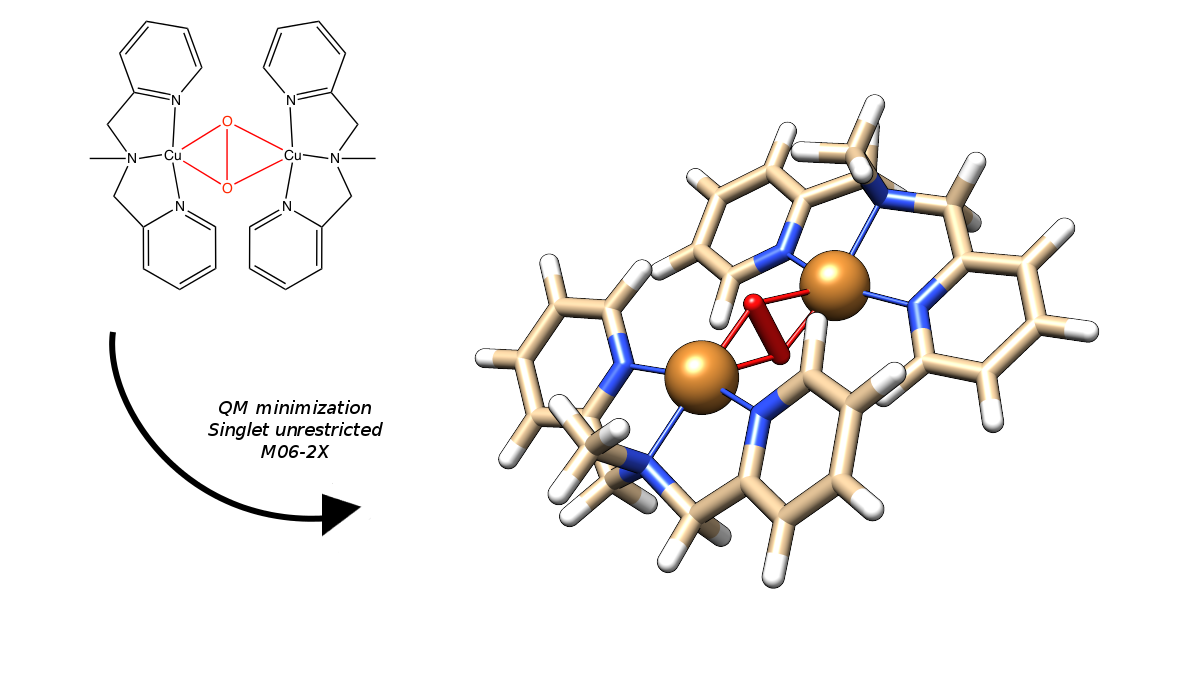
\includegraphics[width=0.9\textwidth]{fig/hemocyanin-qm-minimization.png}}
\caption[Hemocyanin dicopper centre]{Ward's group supplied a draft of the di-copper centre, which was later converted into a standard mol2 file with ChemBio3D. The resulting file was then minimized with Gaussian09 using an M06-2X functional.}
\end{figure}

An initial population of 1000 individuals was created and evolved for 300 generations with a crossover probability of 0.8 and mutation rate of 0.1. Additionally, a main distance objective was asked: the free end of the ligand should approach the terminal-N of the biotin in the other subunit to meet a covalent-suitable distance. An idealization of the final requirements is depicted in figure 4.6.
\begin{figure}
\noindent\makebox[\textwidth][c]{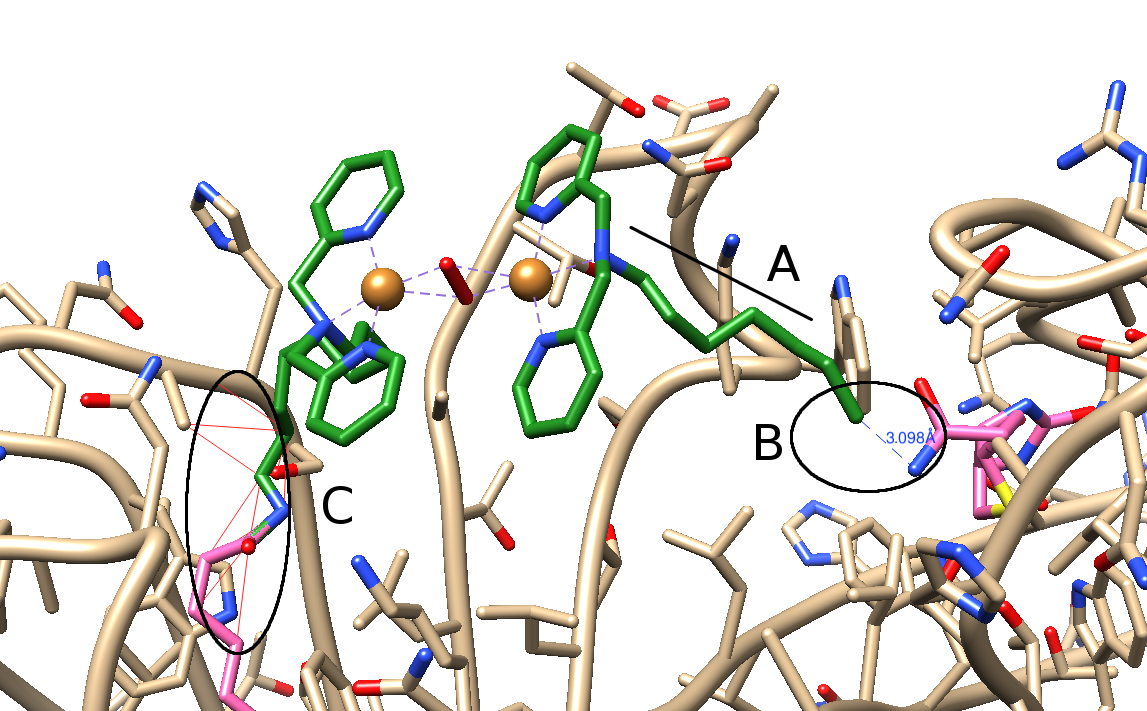
\includegraphics[width=0.9\textwidth]{fig/hemocyanin_objectives.png}}
\caption[Idealization of objectives for the hemocyanin case study]{Partial idealization of required objectives. To obtain a feasible sketch, GAUDI\textsubscript{ASM} was fed with several objectives. The main ones are depicted in this figure. Both linkers are dynamical entities and are represented by an alkyl chain of a variable number of carbons (from 3 to 9). The number of carbons and their torsion angles (A) were optimized to meet a covalent distance objective between the terminal atom of the molecule and the terminal N of the 2nd biotin (B), while minimizing steric clashes (C) and maximizing Van der Waals interactions (not shown).}
\end{figure}


%___________________________________________________________________________

\section*{\phantomsection%
  4.4. Discussion of results%
  \addcontentsline{toc}{section}{4.4. Discussion of results}%
  \label{discussion-of-results}%
}

The resulting Pareto front consisted of 1599 individuals, a selection of which was extracted following these score constrains in GaudiView GUI:
%
\begin{quote}
%
\begin{itemize}

\item Clashes < 20 nm³\footnote{Due to an artifact in the clash detection engine, the first covalent interaction does account for ~10nm³. As a result, this upper limit would allow a second covalent interaction as the maximum tolerated overlapping.}

\item Distance to biotin < 2.0 A\footnote{The length of a single C-N bond is usually around 1.5A. Setting the limit up to 2.0A allows some flexibility in the results.}

\end{itemize}

\end{quote}

What we first observed is that the needed length for the linker should go beyond the five-carbon linker that experimentalists were trying. In fact, according to the results, the linkers should contain between six and eight carbons each, thus favouring a 7C-symmetrical construction (see figure 4.7). Also, one candidate solution feature an eight-plus-four construction, suggesting that it could be enough with six carbons in each linker (still above the length tested experimentally).

However, with such length, we would expect an excessive flexibility in the system, which suggests the use of some rigidifying modifications, such as inserting some unsaturations in the linker. We also observed some undesired hydrophobic interactions between the linkers and the inner faces of the binding cavity that prevented the system from reaching the second biotin. The addition of some polar groups to the linker is thus suggested.

While the proposed solutions have slightly different orientations, all of them were able to find a cavity in the interface of the monomers of the dimeric subunit of streptavidin, as it can be seen of figure 4.8.

\begin{table}[h]
\centering
\caption{Selected hemocyanin poses.}
\label{my-label}
\begin{tabular}{@{}llllll@{}}
\toprule
Model & Linker A  & Linker B  & Distance to biotin & Clashes (nm³) & Contacts \\ \midrule
277   & 8 carbons & 6 carbons & 1.809 A            & 10.6661       & 14.4928  \\
479   & 8 carbons & 6 carbons & 2.437 A            & 14.6741       & 25.4074  \\
187   & 8 carbons & 6 carbons & 2.652 A            & 9.46732       & 18.1877  \\
265   & 8 carbons & 4 carbons & 1.803 A            & 10.5548       & 18.4069  \\ \bottomrule
\end{tabular}
\end{table}
\begin{figure}
\noindent\makebox[\textwidth][c]{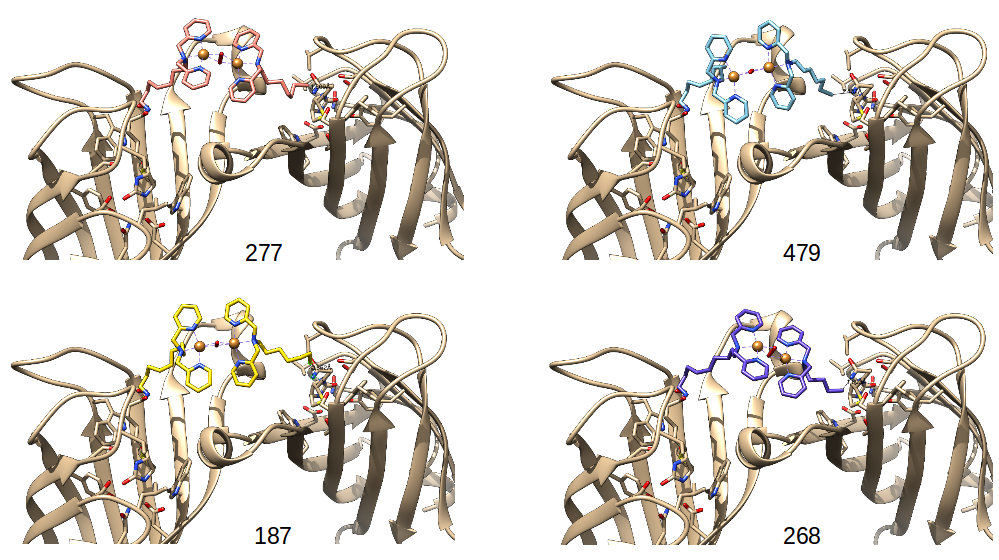
\includegraphics[width=0.9\textwidth]{fig/results-hemocyanin.png}}
\caption[Proposed solutions for the hemocyanin case study]{The four selected poses reveal different linker configurations while maintaining a similar pattern in the location of the core.}
\end{figure}

\begin{figure}
\noindent\makebox[\textwidth][c]{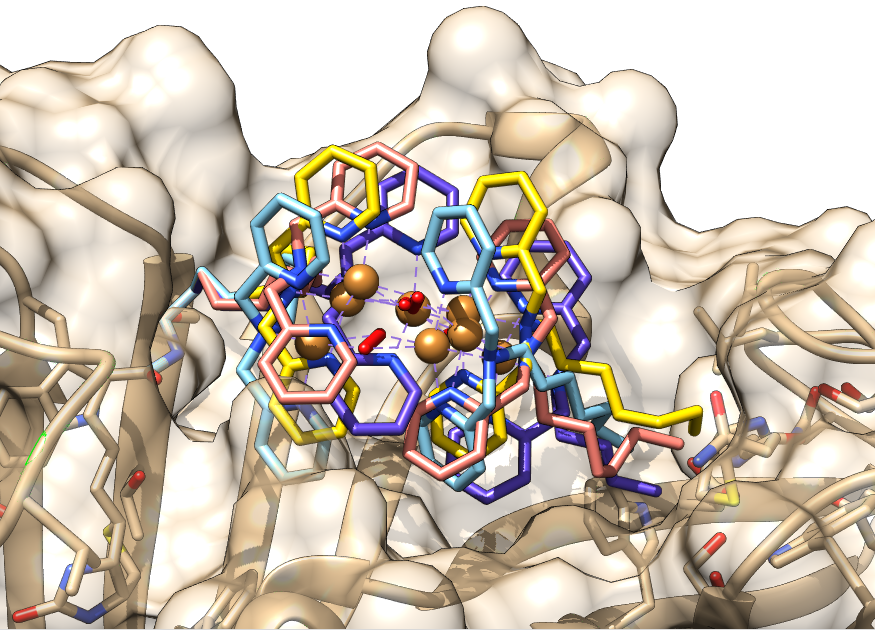
\includegraphics[width=0.9\textwidth]{fig/hemocyanin-solutions-cavity.png}}
\caption[A suitable cavity was found in the monomers interface of hemocyanin]{ The steric clashes detection engine allows easy recognition of the conformational space and provides physically sound compound poses. Here, the hemocyanin construction found a feasible cavity in the interface of the two monomers that compose the dimeric subunit of streptavidin.}
\end{figure}


%___________________________________________________________________________

\subsection*{\phantomsection%
  Conclusions%
  \addcontentsline{toc}{subsection}{Conclusions}%
  \label{conclusions}%
}

Even at a early stage of development, GAUDI\textsubscript{ASM} has proved it can shed light on the problems that experimentalists are facing. A simple essay that took less than two hours revealed the main obstacle they were struggling with: the length of the linkers was insufficient.

It also provided a visual picture of the system, and pointed out some of the difficulties they will have to deal: how would the system behave in a deoxygenated state? It will probably suffer from excessive chain movement, and resolving that issue may imply additional anchoring to the inner sides of the cavity. Further studies will be focusing on the approach of the side carbons in the N-rings of the copper scaffolds to residues K109 and K233, which may be able to facilitate additional anchoring to help fix the long chain.


\chapter{Case Study II: Aluminium}%


%___________________________________________________________________________

\section*{\phantomsection%
  5.1. Metals and life%
  \addcontentsline{toc}{section}{5.1. Metals and life}%
  \label{metals-and-life}%
}

As it was advanced in the previous chapter, metals play an important role in several biological processes. They are central to a lot of essential biological reactions, but they can also be very toxic. As enunciated by Paracelsus, it's the dose that makes the poison. Life processes are very sensitive to concentration changes, especially when it comes to metal ions. As a result, if blood levels of a given metal experiments a sudden increase or decrease of concentration, it can lead to devastating consequences. For example, the most common case of anaemia is caused by iron deficiency: without iron, the cells cannot form enough functional haemoglobin to bind oxygen and support their metabolism.

Besides their metabolic implications, anomalies in the homeostasis of some metals have been reported to participate in some neurodegenerative disorders, such as Parkinson's (PD) or Alzheimer's (AD) disease. While AD is characterized by the accumulation of amyloid-beta plaques in the brain, its true etiology remains unknown. Aluminium has been in the spotlight since its brain accumulation was first described by \DUrole{citein}{Crapper1973}, amongst other metals \DUrole{cite}{Shcherbatykh2007, Gonzalez-Dominguez2014}. Although mainstream science seems to have abandoned the aluminium hypothesis due to some controversy in the previous studies \DUrole{cite}{Santibanez2007}, it still attracts scientists \DUrole{cite}{Lidsky2014}.


%___________________________________________________________________________

\subsection*{\phantomsection%
  5.1.1. Aluminium as a biometal%
  \addcontentsline{toc}{subsection}{5.1.1. Aluminium as a biometal}%
  \label{aluminium-as-a-biometal}%
}

Aluminium, despite its relatively high abundance, is barely used in living organisms. However, the increase of its concentration in our environment had made its interaction with biological material more frequent. In spite of all this, its actual binding capabilities are rather puzzling.

Aluminium(III) can coordinate to several different elements, but it particularly leans towards nitrogen and oxygen atoms in biological environments \DUrole{cite}{Kaim1994}, though oxygen is preferred due to its smaller size and larger negative charge. Thus, in a proteic environment, it will mostly bind to aspartic and glutamic acids, serine residues and the oxygens found in the backbone. The resulting complexes tend to feature coordination numbers of four, five and six \DUrole{cite}{GreenWood1997}, which usually means \emph{trigonal planar, tetrahedral, trigonal bipyramidal, and octahedral geometries}.


%___________________________________________________________________________

\section*{\phantomsection%
  5.2. The challenge%
  \addcontentsline{toc}{section}{5.2. The challenge}%
  \label{the-challenge}%
}

In collaboration with the group of Prof. Xabier López at the UPV/EHU, our group aims at identifying the mechanism under which aluminium interacts with b-amyloids and generate three dimensional models of the most likely binding modes of coordination. After having explored under quantum mechanical studies cluster models limited to the first coordination of the metal that Al(III) prefers, coordination that involved three to four carboxyl containing residues, GAUDI was used to satisfy those criteria under a proteic environment.

A first filtering of all the b-amyloid structures available in the PDB was performed considering the optimized position of alpha-carbons of all acidic residues and carbonyl side chains of the experimental structures. GRID-optimized systems obtained from the PDB screening resulted in PDB entries 1AMB, 1AMC, 1AML, 1BA4, 1BA6, 1BJB, 1BJC, 1IYT, 1NMJ, 1Z0Q, 2LFM, 2M9R, and 2M9S. GAUDI\textsubscript{ASM} objectives were therefore to find the nearby oxygen-containing residues and optimize their rotameric configuration so they can allocate the aluminium in a feasible coordination geometry. Backbone oxygen atoms were also allowed to participate in the complex.


%___________________________________________________________________________

\section*{\phantomsection%
  5.3. Current techniques in bioinformatics%
  \addcontentsline{toc}{section}{5.3. Current techniques in bioinformatics}%
  \label{current-techniques-in-bioinformatics}%
}

This case study can be regarded as a docking problem where the ligand is a single atom of aluminium. However, existent docking solutions rarely accept metals in the input, let alone being the naked ligand. Furthermore, rotameric optimization programs are usually directed towards hydrogen bond forming, Van der Waals contacts, and avoiding clashes, not towards the discovery of suitable coordination geometries. GOLD does implement this feature but is not optimized to handle them as part of the ligand \DUrole{cite}{Ortega-Carrasco2014}, and so does FlexX \DUrole{cite}{Seebeck2008}, but it does not support naked metal ions as ligands. Since GAUDI\textsubscript{ASM} can be easily extended to adopt new objectives and features, we thought of creating an alternative launcher script that would meet the requirements of this essay.


%___________________________________________________________________________

\section*{\phantomsection%
  5.4. Our strategy%
  \addcontentsline{toc}{section}{5.4. Our strategy}%
  \label{our-strategy}%
}

GAUDI\textsubscript{ASM} can treat any UCSF Chimera compatible input file as a ligand, so using a single aluminium atom as a ligand works out of the box. However, the provided dataset already included a tentative position for the aluminium, making that step unnecessary. Instead, the new script only had to detect existent aluminium atoms and register them as ligands. If more than one were found, only the one with the lowest serial number would be taken into account.
\begin{figure}
\noindent\makebox[\textwidth][c]{\includegraphics[width=0.9\textwidth]{fig/pseudo-al.pdf}}
\caption[Aluminium script pseudocode]{Pseudocode for the aluminium case study. This is slightly different from the GAUDI\textsubscript{ASM} launcher script, but uses the same framework.}
\end{figure}

Once found, the initial set-up was performed. Since each of the 13 PDB entries contained several different poses, which in total accounted for 157 possible input files, a complementary helper script was designed to run all of them in batch. Each of the essays started with a population of 300 individuals and ran for 15 generations, with mu, lambda, and crossover probability set to 0.5, and mutation rate set to 0.2.

In each essay, the aluminium was allowed to move to a random point within 2.5A of the starting position, and then search space field was created within 7.0A of the new position. If one or more oxygen atoms were found in the search sphere, their correspondent residues were registered in the rotamers optimization list. It mostly comprised aspartic and glutamic acids, and some serines too.

Detecting feasible coordination geometries can be an attractive feature and definitely will be implemented in the future, but for this essay it was not necessary. After choosing a new set of rotamers from the Dunbrack's library, the distances of the three nearest oxygen atoms were calculated, as well as the standard and dihedral angles that their two immediate neighbours, themselves, and the aluminium ion formed. GAUDI\textsubscript{ASM} was then set up to minimize both the distances to 2.2A with a minimum distance threshold of 1.8A, and the absolute sine of each of the dihedrals, seeking to obtain information about the planarity requirements of the coordinate residue, be it mono or bidentate. In order to avoid infeasible steric conformations, the clashes were calculated and minimized too.
\begin{figure}
\noindent\makebox[\textwidth][c]{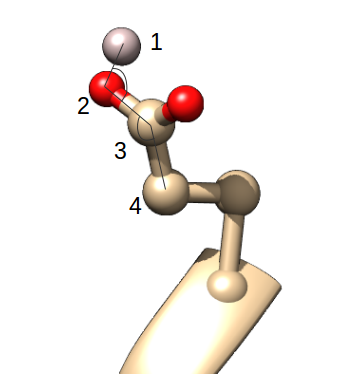
\includegraphics[width=0.6\textwidth]{fig/dihedral.png}}
\caption[Dihedral angle calculation]{The directionality of the coordination interaction is expressed as the absolute sine of the dihedral angle formed between the atoms 1, 2, 3, and 4; also, the absolute sine of the angle formed between 1, 2, and 3 is taken into account. An absolute sine of zero means perfect alignment, while an absolute sine of one means perfect perpendicularity.}
\end{figure}

Last but not least, an additional scoring was added to account for the number of oxygen-containing residues found within 2.0A from the aluminium atom, which would give an approximate idea of the coordination number.

\vspace*{\fill}
\newpage
%___________________________________________________________________________

\section*{\phantomsection%
  5.5. Discussion of results%
  \addcontentsline{toc}{section}{5.5. Discussion of results}%
  \label{discussion-of-results}%
}

The generated Pareto front of solutions comprised more than 19,000 possible candidates, so an obvious filtering was needed. These were the applied restrictions.

\begin{itemize}

\item Clashes < 10 nm³

\item At least two oxygen atoms within 2.0A from the aluminium

\end{itemize}

This configuration left us with 11 solutions. Of these 11, a total of five poses were chosen and proposed to Xabier. These were based on PDB entries 1AMC, 1AML, 1BJB, 1BJC, and 1Z0Q, whose details can be read in table 5.1. As it can be seen, the poses tend to feature three or four proximal oxygen atoms that would suggest an octahedral geometry. These atoms usually come from the carboxylic group of aspartic and glutamic acids, though some oxygen atoms from the atom can be also pointed out.
\begin{figure}
\noindent\makebox[\textwidth][c]{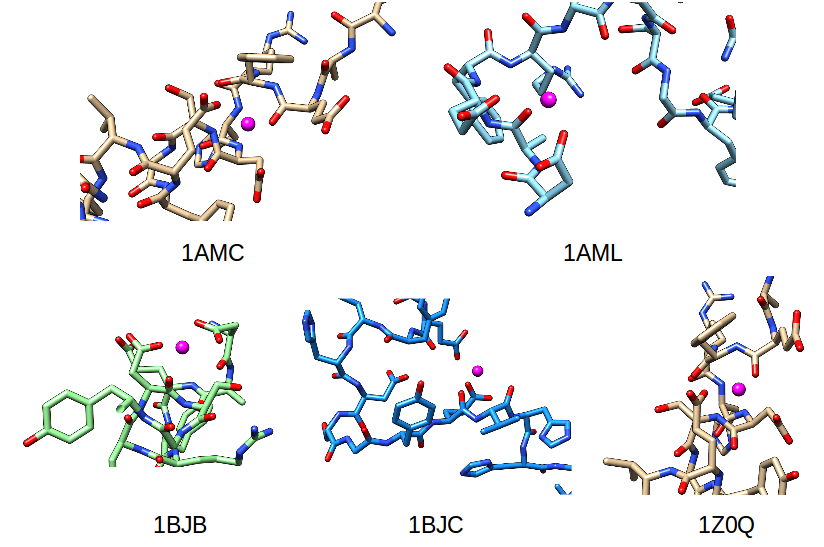
\includegraphics[width=0.9\textwidth]{fig/results-aluminium.png}}
\caption[Selected solutions in the aluminium case study]{Selected solutions from the Pareto front proposed by the GAUDI\textsubscript{ASM} essay. Aluminium ions are depicted in bright magenta.}
\end{figure}

\begin{table}[h]
\centering
\caption[Scoring of each proposed solution for the aluminum case study]{Details of the scoring of each proposed solutions. \emph{Nearby oxygens} refers to the number of oxygen atoms within 2.2A of the aluminium ion. \emph{Average distance} is calculated from the distance of the three nearest oxygens to the aluminium ion. \emph{Average planarity} is the mean of the absolute sines of the dihedrals formed with aluminium, oxygen, and the next two non-terminal atoms in the peptidic chain. A planarity of zero means that the chains are aligned, while a planarity of one means they are orthogonal. More details are given in Appendix A.}
\label{my-label}
\resizebox{\textwidth}{!}{%
\begin{tabular}{@{}lllll@{}}
\toprule
PDB code & Nearby oxygens & Clashes (nm³) & Average distance (nm) & Average planarity \\ \midrule
1AMC & 2 & 7.8922 & 2.6789 & 0.6433 \\
1AML & 2 & 6.1656 & 2.3198 & 0.9189 \\
1BJB & 2 & 7.6941 & 2.2176 & 0.5629 \\
1BJC & 2 & 8.1273 & 2.3761 & 0.8315 \\
1Z0Q & 2 & 9.665 & 2.3291 & 0.7289 \\ \bottomrule
\end{tabular}
}
\end{table}


%___________________________________________________________________________

\subsection*{\phantomsection%
  Conclusions%
  \addcontentsline{toc}{subsection}{Conclusions}%
  \label{conclusions}%
}

GAUDI\textsubscript{ASM} has to allow dealing with metal coordination as one requirement in many new chemobiological experiments. The first functionality along this line have been incorporated in the program and, thanks to the initial inputs provided by Prof. López group, we applied this tool to the binding of aluminium to a peptide. Simple geometric parameters like threshold distances, angles and dihedrals have reported interesting results, raising our interest in this unexplored field of docking experiments. As a result, a more advanced and very promising predictive engine is already under development.


\chapter{Conclusions}



%___________________________________________________________________________

\section*{\phantomsection%
  Conclusions%
  \addcontentsline{toc}{section}{Conclusions}%
  \label{conclusions}%
}

GAUDI has proved to be a valid proof of concept. Simplistic energy calculation terms do generate good results if combined with the appropriate restraints, which is one of the most powerful strengths of this software. It can help molecular designers with a rapid sketching tool that will produce feasible in results in a reasonable amount of time.


%___________________________________________________________________________

\section*{\phantomsection%
  Further work%
  \addcontentsline{toc}{section}{Further work}%
  \label{further-work}%
}
%
\begin{itemize}

\item Further development of the spatial exploration engine: improve free docking results, global protein flexibility

\item More objectives: Metal coordination geometries prediction (not just visual aid)

\item QM/MM minimization interface from GaudiView: direct refinement from the GUI

\item Performance improvements: parallelization, code polish

\item Custom %
\raisebox{1em}{\hypertarget{id2}{}}\hyperlink{id1}{\textbf{\color{red}*}}.frcmod inputs as energy terms

\end{itemize}




\begin{appendices}
	\renewcommand\chaptername{Appendix}
    \chapter{Programmatic details}%



%___________________________________________________________________________

\section*{\phantomsection%
  A.1. Language and development environment choices%
  \addcontentsline{toc}{section}{A.1. Language and development environment choices}%
  \label{a-1-language-and-development-environment-choices}%
}

Python is a high-level scripting language that allows rapid prototyping. It provides object-oriented programming capabilities but does not compel you to use them. This allows the beginner programmer to combine procedural and OOP styles without any problems, and GAUDI takes advantage of it: the simpler modules are just a collection of related functions, while the most complex ones fully rely on Python classes and objects.

Thus, Python is usually regarded as one of the easiest languages to learn. Furthermore, its compulsory indentation syntax enforces code readability. Since Chimera and DEAP are both open-source, this former characteristic has helped understand a lot of the code patterns that happen behind the scenes of a molecular visualization tool and an evolutionary programming framework, respectively.

UCSF Chimera is developed by the Resource for Biocomputing, Visualization, and Informatics, in the University of California, San Francisco (supported by NIGMS P41-GM103311). It is defined by its authors as \emph{a highly extensible program for interactive visualization and analysis of molecular structures and related data, including density maps, supramolecular assemblies, sequence alignments, docking results, trajectories, and conformational ensembles}. UCSF Chimera includes a lot of Python packages that behave as \emph{plugins} that extend its base functionality. Besides providing GAUDI with a robust visualization tool and a three-dimensional canvas, some of those plugins have been been incorporated into the GAUDI core, such as the H Bond discovery utility or the clashes and contacts detector.

However, UCSF Chimera does not carry a built-in evolutionary algorithm, that's why an additional package was needed. DEAP stands for Distributed Evolutionary Algorithms in Python and, in words from its authors, is \emph{a novel evolutionary computation framework for rapid prototyping and testing of ideas that seeks to make algorithms explicit and data structures transparent}. It provides GAUDI with the main GA engine, whose high customizability has allowed to implement very complex data structures, as required by a molecular design problem. Its transparent approach, as opposed to the majority of the other available evolutionary frameworks, has allowed us to design custom individuals that can confront the design challenge with agility. A typical GAUDI individual includes information about the building blocks and the resultant molecule, its torsion angles, the protein cavity chemical environment or the Cartesian transformation matrices, among others. However, since some GAUDI essays do not need torsion angles or rotamer changes, the GA individuals must be dynamical and only include what is needed in each case, and DEAP has proved to be invaluable in that matter.


%___________________________________________________________________________

\section*{\phantomsection%
  A.2. Main features of GAUDI%
  \addcontentsline{toc}{section}{A.2. Main features of GAUDI}%
  \label{a-2-main-features-of-gaudi}%
}


%___________________________________________________________________________

\subsection*{\phantomsection%
  A.2.1. Hydrogen bonds discovery%
  \addcontentsline{toc}{subsection}{A.2.1. Hydrogen bonds discovery}%
  \label{a-2-1-hydrogen-bonds-discovery}%
}

Possible hydrogen bonds are calculated with the built-in Chimera extension \texttt{FindHBonds}, which in turn is based on the studies by \DUrole{citein}{Mills1996}. Mills et al surveyed the Cambridge Structural Database to derive real-life information about the distances, angles and atoms implied in ligand-receptor interaction. The implementation in Chimera allows to specify a tolerance threshold for both angle and distance, relaxing the geometrical constraints. By default, these have been set to 20 degrees and 0.4 Angstrom, respectively.

In the current implementation, it only serves as a qualitative indicator of how many hydrogen bonds could be formed in the current state. Also, a set of \emph{preferred} H-bond-forming atoms can be specified in the input. If the user decides so, it will account for an extra objective that will be maximized. This allows to use the existent literature and knowledge on the system to perform some prioritization on the protein atoms that could be implied in forming a hydrogen bond.


%___________________________________________________________________________

\subsection*{\phantomsection%
  A.2.2. Clashes and contacts detection%
  \addcontentsline{toc}{subsection}{A.2.2. Clashes and contacts detection}%
  \label{a-2-2-clashes-and-contacts-detection}%
}

Both types of interactions are calculated with the same built-in Chimera extension \texttt{DetectClash}. The base implementation only detects which atoms are within a set threshold from each other. GAUDI extends this basic functionality with some approximative functions based on the distance between the involved atoms.

A \emph{contact} score is defined by a 12-6 Lennard-Jones-like expression which takes the form of:
%
\begin{equation*}
LJS = (\frac{z}{d})^{12} - 2(\frac{z}{d})^6
\end{equation*}
, where $z = 0.98*(r_a + r_b)$, being $r_a$ and $r_b$ the radii of the two involved atoms, and $d$ the distance between them. Since this LJ-like expression takes no constants, no units are provided.

To calculate the clashes, a different strategy is used. The reasoning behind this is founded on the need of a more sensitive method to quantify the clashing. Lennard-Jones approaches tend to be quite harsh on the clash part, so a more soft approach was needed. Thus, the \emph{clash} scores are calculated as the overlapping volume of the Van der Waals spheres of the involved atoms. The volume is calculated analytically as proposed by \DUrole{citein}{Eyal2004}:
%
\begin{equation*}
V_ab = \frac{1}{3} \pi h^2_a(3R_a-h_a) + \frac{1}{3} \pi h^2_b(3R_b - h_b)
\end{equation*}
, where $h_a = \frac{R^2_b - (d - R_a)^2}{2d}$, $h_b = \frac{R^2_a - (d - R_b)^2}{2d}$ if $(d < R_a + R_b)$, and $h_a = h_b = 0$, if $(d \ge R_a + R_b)$. This means the clash score is expressed in $nm^3$.


%___________________________________________________________________________

\subsection*{\phantomsection%
  A.2.3. Solvent accessible and excluded surface area calculation%
  \addcontentsline{toc}{subsection}{A.2.3. Solvent accessible and excluded surface area calculation}%
  \label{a-2-3-solvent-accessible-and-excluded-surface-area-calculation}%
}

Solvent accessible and excluded surface areas (SASA and SESA, respectively) are calculated using the MSMS package \DUrole{cite}{Sanner1996} and the built-in Chimera Python interface. Both SAS and SES areas shed light on solvation and desolvation terms, but SASA seems to be more commonly used when computing desolvation energies due to their strong linear relationship \DUrole{cite}{Wang2002,Dynerman2009}. At any case, GAUDI supports both kinds of areas and it's up to the researcher to choose between maximizing SESA or minimizing SASA.
\begin{figure}
\noindent\makebox[\textwidth][c]{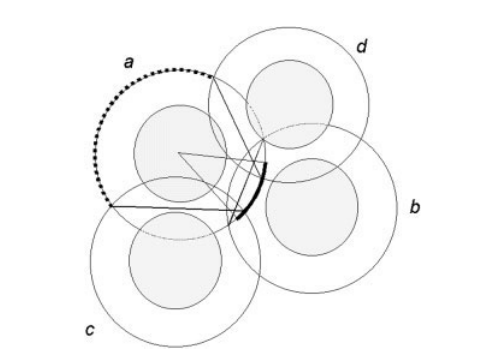
\includegraphics[width=0.6\textwidth]{fig/sasa.png}}
\caption[Solvent accesible surface area and solvent excluded surface area]{Solvent accesible surface area (SASA) and solvent excluded surface area (SESA). \DUrole{cite}{Eyal2004}}
\end{figure}


%___________________________________________________________________________

\subsection*{\phantomsection%
  A.2.4. Meeting a distance objective%
  \addcontentsline{toc}{subsection}{A.2.4. Meeting a distance objective}%
  \label{a-2-4-meeting-a-distance-objective}%
}

This is probably the simpler method implemented in GAUDI, but also one of the more powerful. Given a list of ligand atoms (\texttt{probes}) and a protein atom (\texttt{target}), it will optimize the average distance of each \texttt{probe} and the \texttt{target}. Atoms must be provided using their serial numbers. Furthermore, a special keyword \texttt{last} is also available, and it represents the terminal atom of the ligand; i.e., the \texttt{acceptor} atom with the highest serial number, as defined in the \texttt{attr} file. See section 7 for more information.


%___________________________________________________________________________

\subsection*{\phantomsection%
  A.2.5. Flexibility of the ligand%
  \addcontentsline{toc}{subsection}{A.2.5. Flexibility of the ligand}%
  \label{a-2-5-flexibility-of-the-ligand}%
}

Flexibility on the ligand is achieved by taking advantage of the torsion handlers in the core \texttt{BondRot} package of Chimera. The engine has been modified to detect amide bonds -{}- these kind of bonds are only able to flip in a cis/trans fashion -{}- and in-cycle bonds, which cannot be rotated.

GAUDI supports partial flexibility, so it is possible to specify a maximum amount of torsion the ligand bonds cannot exceed. Thanks to simulated binary crossovers and mutations, there's no need to represent the torsion chromosomes as a binary string. This allows to achieve float precision for every torsion angle \DUrole{cite}{Deb1995}, if needed. GOLD, on its behalf, uses a pure binary string in which each byte encodes a torsion angle. This approach allows allows a precision of 1.4 degrees \DUrole{cite}{Jones1997}.


%___________________________________________________________________________

\subsection*{\phantomsection%
  A.2.6. Rotamer and mutation retrieving%
  \addcontentsline{toc}{subsection}{A.2.6. Rotamer and mutation retrieving}%
  \label{a-2-6-rotamer-and-mutation-retrieving}%
}

UCSF Chimera offers a Python interface to Dunbrack's \DUrole{cite}{Dunbrack1994} and Dynameomics \DUrole{cite}{Scouras2011} rotameric libraries. Both libraries are sorted by the observed frequency of each rotamer, so, given a residue type with phi and psi angles, every rotamer can be unequivocally accessed using an index. Thus, two parallel lists are maintained as separated genes: rotamer indices for every requested residue position, and, in the case of random mutations are allowed, the corresponding indices to a list that holds the requested mutation types. As for the genetic operators, GAUDI also performs simulated binary crossover and mutation on this two former genes.


%___________________________________________________________________________

\subsection*{\phantomsection%
  A.2.7. Space exploration and recombination%
  \addcontentsline{toc}{subsection}{A.2.7. Space exploration and recombination}%
  \label{a-2-7-space-exploration-and-recombination}%
}

Though GAUDI's primary objective is not directed towards classic docking essays, it does provide a simple exploration engine that can greatly extend the design opportunities. In its approach, GAUDI makes use of two independent transformation matrices: one contains the translation info, while the other addresses the rotation parameters.

If a recombination event takes place, the matrices from each parent are multiplied and then, the two resulting matrices are interpolated to produce an intermediate transform which is later decomposed back into its translation and rotation components. The two new individuals inherit one matrix from one of the parents, and one from the interpolated matrix. Mutation is handled in a simpler fashion: the new matrices are generated randomly from scratch, as in the initial population setup.


%___________________________________________________________________________

\subsection*{\phantomsection%
  A.2.8. Ligand building%
  \addcontentsline{toc}{subsection}{A.2.8. Ligand building}%
  \label{a-2-8-ligand-building}%
}

UCSF Chimera provides no simple mechanism to build molecules interactively, let alone programmatically. It does include a package called \texttt{BuildStructure}, but its current implementation is insufficient. GAUDI solves this lack with two custom classes: \texttt{Molecule.Library} and \texttt{Molecule.Compound}. A \texttt{Compound} object can be instantiated from an existent \texttt{Chimera.Molecule} object or any file that Chimera can open. It provides several useful novel methods, such as \texttt{append()} or \texttt{place()}. This allows to block-build a custom ligand just by appending several molecules on top and place the result in an adequate pose for later manipulation.

In order to properly handle the constructions, a separate \texttt{attr} file or Python dictionary must be provided. These attributes determine which atoms in the building block correspond will behave as an acceptor, donor, respectively. It can also contain a set of bonded atom pairs whose bond should not be rotated. These special roles are needed for the extended functionality of the \texttt{Compound} class. For example, the \texttt{append()} method will join the \texttt{donor} atom of the new molecule to the \texttt{acceptor} atom of the already present molecule.

The \texttt{Library} class was designed to implement lazy loading. If GAUDI were to hold all the ligands that can be built from the input blocks, it would soon run out of memory and crash -{}- especially considering how memory intensive Chimera tends to be \DUrole{cite}{ChimeraMemoryUsage}. Subsequently, the \texttt{Library} handles \texttt{Compound} objects creation and required elongations on a per-request basis.


%___________________________________________________________________________

\subsection*{\phantomsection%
  A.2.9. Input and output files%
  \addcontentsline{toc}{subsection}{A.2.9. Input and output files}%
  \label{a-2-9-input-and-output-files}%
}

GAUDI uses YAML-formatted files for both input and output files. The parsing is done with an external package called PyYAML \DUrole{cite}{PyYAML}. YAML is a human-readable serialization format, already implemented in a broad range of languages \DUrole{cite}{Yaml2009}. Formally, GAUDI files consists of a number of dictionaries, whose values are dictionaries themselves. However, due to YAML high readability, it looks just like a typical indented list. This an excerpt from a sample input:
%
\begin{quote}{\ttfamily \raggedright \noindent
protein:\\
~~~~path:~/home/jr/x/hyde/mol2/ethanol.mol2\\
~~~~origin:~5\\
~~~~radius:~10.0\\
~\\
ligand:\\
\#~if~a~path~is~submitted,~all~combinations~will~be~generated\\
~~~~path:~/home/jr/x/03\_\_projects/hemocyanin/input\_no\_subst/\\
~~~~type:~blocks\\
~~~~flexibility:~360\\
~~~~bondto:~1868\\
~\\
rotamers:\\
~~~~residues:~{[}233,~109{]}\\
~~~~library:~dynameomics\\
~~~~top:~8\\
~~~~mutate:~no\\
~\\
objectives:\\
~~~~-~name:~Clashes\\
~~~~~~type:~contacts\\
~~~~~~which:~clashes\\
~~~~~~weight:~-1.0\\
~~~~~~test:~ligand\\
~~~~~~threshold:~0.4\\
~\\
~~~~-~name:~HBonds\\
~~~~~~type:~hbonds\\
~~~~~~weight:~1.0
}
\end{quote}

The only possible draw-back is that YAML, like Python, has meaningful indentation. This is particularly important in the list of objectives, which is actually a dictionary whose only value is a list (hence the hyphens) of sub-dictionaries. If the indentation is not respected, the parsing will not succeed.

\end{appendices}

\singlespacing

% the back matter
\clearpage
\listoffigures
\addcontentsline{toc}{chapter}{Listing of figures}
\cleardoublepage
\bibliography{references}
\addcontentsline{toc}{chapter}{References}
\bibliographystyle{newapa}
\cleardoublepage

\end{document}
